\documentclass[letterpaper, 10.5pt,landscape]{article}
\renewcommand{\familydefault}{\sfdefault} %% default font
\usepackage{multicol}
\usepackage{calc}
\usepackage{ifthen}

\usepackage[usenames,dvipsnames]{color}  % for text color


\usepackage[landscape]{geometry}
\usepackage[inkscapelatex=false]{svg}


\def\mathcolor#1#{\@mathcolor{#1}}
\def\@mathcolor#1#2#3{%
  \protect\leavevmode
  \begingroup
    \color#1{#2}#3%
  \endgroup
}

\usepackage[
backend=biber,
style=numeric,
sorting=ynt
]{biblatex}
\addbibresource{reference.bib}


\usepackage{ragged2e}
\usepackage{tabularx}


\usepackage{amsmath, amssymb, amsthm}
\usepackage{blkarray} % For block array
\DeclareMathOperator*{\argmin}{argmin}
\usepackage{latexsym, marvosym}
\usepackage{pifont}
\usepackage{lscape}
\usepackage{graphicx}
\usepackage{array}
\usepackage{booktabs}
\usepackage[bottom]{footmisc}
\usepackage{tikz}
\usetikzlibrary{shapes}
\usepackage{pdfpages}
\usepackage{wrapfig}
\usepackage{enumitem}
\setlist[description]{leftmargin=0pt}
\usepackage{xfrac}
\usepackage[pdftex,
            pdfauthor={William Chen},
            pdftitle={Probability Cheatsheet},
            pdfsubject={A cheatsheet pdf and reference guide originally made for Stat 110, Harvard's Introduction to Probability course. Formulas and equations for your statistics class.},
            pdfkeywords={probability} {statistics} {cheatsheet} {pdf} {cheat} {sheet} {formulas} {equations}
            ]{hyperref}
\usepackage[
            open,
            openlevel=2
            ]{bookmark}
\usepackage{relsize}
\usepackage{rotating}

 \newcommand\independent{\protect\mathpalette{\protect\independenT}{\perp}}
    \def\independenT#1#2{\mathrel{\setbox0\hbox{$#1#2$}%
    \copy0\kern-\wd0\mkern4mu\box0}} 
            
\newcommand{\noin}{\noindent}    
\newcommand{\logit}{\textrm{logit}} 
\newcommand{\var}{\textrm{Var}}
\newcommand{\cov}{\textrm{Cov}} 
\newcommand{\corr}{\textrm{Corr}} 
\newcommand{\N}{\mathcal{N}}
\newcommand{\Bern}{\textrm{Bern}}
\newcommand{\Bin}{\textrm{Bin}}
\newcommand{\Beta}{\textrm{Beta}}
\newcommand{\Gam}{\textrm{Gamma}}
\newcommand{\Expo}{\textrm{Expo}}
\newcommand{\Pois}{\textrm{Pois}}
\newcommand{\Unif}{\textrm{Unif}}
\newcommand{\Geom}{\textrm{Geom}}
\newcommand{\NBin}{\textrm{NBin}}
\newcommand{\Hypergeometric}{\textrm{HGeom}}
\newcommand{\HGeom}{\textrm{HGeom}}
\newcommand{\Mult}{\textrm{Mult}}

%%%%%%%%%%%%%%%%%%%%%%
\usepackage{listings}

%New colors defined below
\definecolor{codegreen}{rgb}{0,0.6,0}
\definecolor{codegray}{rgb}{0.5,0.5,0.5}
\definecolor{codepurple}{rgb}{0.58,0,0.82}
\definecolor{backcolour}{rgb}{0.95,0.95,0.92}

%Code listing style named "mystyle"
\lstdefinestyle{mystyle}{
  backgroundcolor=\color{white}, commentstyle=\color{codepurple},
  keywordstyle=\color{blue},
  numberstyle=\tiny\color{codegray},
  stringstyle=\color{codegreen},
  basicstyle=\ttfamily\footnotesize,
  breakatwhitespace=false,         
  breaklines=true,                 
  captionpos=b,                    
  keepspaces=true,                 
  % numbers=left,                    
  % numbersep=5pt,                  
  showspaces=false,                
  showstringspaces=false,
  showtabs=false,                  
  tabsize=1
}

%"mystyle" code listing set
\lstset{style=mystyle}

%%%%%%%%%%%%%%%%%%%%%


\geometry{top=.2in,left=.2in,right=.2in,bottom=.2in}

\pagestyle{empty}
\makeatletter
\renewcommand{\section}{\@startsection{section}{1}{0mm}%
                                {-1ex plus -.5ex minus -.2ex}%
                                {0.1ex plus .2ex}%x
                                {\normalfont\small}}
\renewcommand{\subsection}{\@startsection{subsection}{2}{0mm}%
                                {-1explus -.5ex minus -.2ex}%
                                {0.5ex plus .2ex}%
                                {\normalfont\normalsize\bfseries}}
\renewcommand{\subsubsection}{\@startsection{subsubsection}{3}{0mm}%
                                {-1ex plus -.5ex minus -.2ex}%
                                {1ex plus .2ex}%
                                {\normalfont\small\bfseries}}
\makeatother

\setcounter{secnumdepth}{0}

\setlength{\parindent}{0pt}
\setlength{\parskip}{0pt plus 0.5ex}

% -----------------------------------------------------------------------

\usepackage{titlesec}

\titleformat{\section}
{\color{teal}\normalfont\large\bfseries}
{\color{teal}\thesection}{1em}{}
\titleformat{\subsection}
{\color{teal}\normalfont\normalsize}
{\color{teal}\thesection}{1em}{}
\titleformat{\subsubsection}
{\color{teal}\normalfont\small}
{\color{teal}\thesection}{1em}{}

% Comment out the above 5 lines for black and white

\begin{document}

\raggedright
\footnotesize

\begin{multicols*}{3}

% multicol parameters
% These lengths are set only within the two main columns
%\setlength{\columnseprule}{0.25pt}
\setlength{\premulticols}{1pt}
\setlength{\postmulticols}{1pt}
\setlength{\multicolsep}{1pt}
\setlength{\columnsep}{2pt}

%%%%%%%%%%%%%%%%%%%%%%%%%%%%%%%%%%%%
%%% TITLE
%%%%%%%%%%%%%%%%%%%%%%%%%%%%%%%%%%%%

\begin{center}
    {\color{teal} \Large{\textbf{Machine Learning Cheatsheet}}} \\
   % {\Large{\textbf{Probability Cheatsheet}}} \\
    % comment out line with \color{blue} and uncomment above line for b&w
   \copyright \ 2024 \  Robins Yadav
\end{center}



% Cheatsheet format from
% http://www.stdout.org/$\sim$winston/latex/

%%%%%%%%%%%%%%%%%%%%%%%%%%%%%%%%%%%%
%%% BEGIN CHEATSHEET
%%%%%%%%%%%%%%%%%%%%%%%%%%%%%%%%%%%%














%%%%%%%%%%%%%% Machine Learning %%%%%%%%%%%%%%%%%%%%%%%%%%%%%%%%%%%%%
\section{Machine Learning General} {\color{teal}\hrule height 1pt} \smallskip
\subsubsection{Definiton} {\color{teal}\hrule height 0.5pt} \smallskip

We want to learn a target function $f$ that maps input
variables $X$ to output variable $y$, with an error $e$:
\vspace{-5pt}
\[\boxed{y = f(X) + e}\]

\subsubsection{Linear, Non-linear} {\color{teal}\hrule height 0.5pt} \smallskip

Different algorithms make different assumptions about the
\textbf{shape} and \textbf{structure} of $f$. Any algorithm can be either:
\begin{itemize}
    \item \textbf{Paramteric (or Linear)}: simplify the mapping to a known linear combination form and learn its coefficients.
    \item \textbf{Non-parametric (or Non-linear):} free to learn any functional form from the training data, while maintaining some ability to generalize.
\end{itemize}

\textbf{\textcolor{blue}{Note: }} Linear algorithms are usually simpler, faster and requires
less data, while Nonlinear can be are more flexible, more powerful and more performant.

\subsubsection{Supervised, Unsupervised} {\color{teal}\hrule height 0.5pt} \smallskip

$\bullet$ \textbf{Supervised} learning methods learn to predict outcomes $y$ (\(y^{(1)}, ..., y^{(m)}\)) from data points $X$ (\(x^{(1)}, ..., x^{(m)}\)) given that the \textbf{data is labeled}. \\

$\rightarrow$ \textbf{Type of prediction}
\vspace{-5pt}
\begin{center}
        \footnotesize
        \scalebox{0.9}{
        \begin{tabularx}{3.5in}{X|X|X}
          & \textbf{Regression} & \textbf{Classification} \\
         \hline
         \textbf{Outcome} & Continuous & Class \\
         \hline
         \textbf{Examples} & Linear Regression & Logistic Regression, SVM, Naive Bayes\\
         \hline
        \end{tabularx}}
\end{center}

\vspace{-3pt}
$\rightarrow$ \textbf{Conditional Estimates} \\
Regression $\rightarrow$ \textbf{conditional expectation}: \(E \left[y|X=x \right] \) \\
Classification $\rightarrow$ \textbf{conditional probability}: \(P(Y=y | X=x) \)

\vspace{3pt}
$\bullet$ \textbf{Unsupervised} learning methods learn to find the inherent structure or hidden patterns from \textbf{unlabeled data} 
 $X$ (\(x^{(1)}, ..., x^{(m)}\)) . 


\subsubsection{Type of models} {\color{teal}\hrule height 0.5pt} \smallskip

$\rightarrow$ \textbf{Discriminative Model}: It focuses on predicting the data's outputs (for classification or regression) by training a model. It learns parameters by maximizing the \textbf{conditional probability} $P(Y|X)$.

\vspace{2pt}

$\rightarrow$ \textbf{Generative Model}: It focuses on learning a probability distribution for the dataset, it can reference this probability distribution to generate new data instances. It learns parameters by maximizing the \textbf{joint probability} of $P(X, Y) = P(X \cap Y)$ .
\vspace{-5pt}

\vspace{-5pt}
\begin{center}
    \begin{minipage}{0.8\linewidth}
    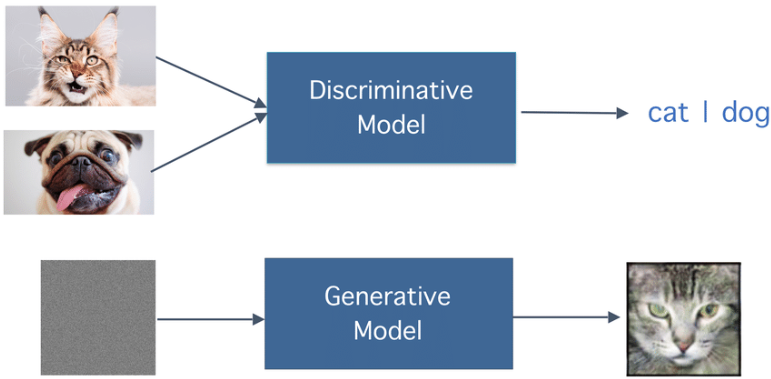
\includegraphics[width=\textwidth]{figures/Discriminant_Generative_Illustration.PNG}
    \end{minipage}
\end{center}
\vspace{-7pt}





\vspace{-7pt}



\begin{center}
    \footnotesize
    \scalebox{0.9}{
    \begin{tabularx}{3.5in}{X|X}
    \textbf{\textcolor{purple}{Discriminative model}} & \textbf{\textcolor{purple}{Generative model}}\\
    \hline
    \RaggedRight{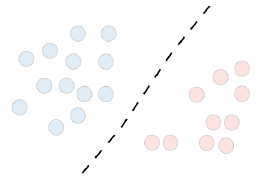
\includegraphics[scale = .40]{figures/Discriminant_model_figure.PNG}}&
    \RaggedRight{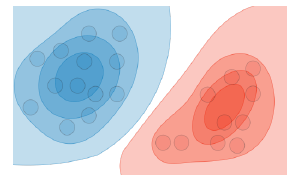
\includegraphics[scale = .36] {figures/Generative_model_figures.PNG}} \\
    \hline
    Learns the decision boundary between classes &
    Learns the input distribution \\
    \hline
    Directly estimate $P(y|x)$ &
    Estimate $P(x|y)$ to find likelihood $P(y|x)$ using \textbf{Baye's} rule \\
    % \hline
    % Cannot generate new data &
    % {Can be used to generate new data} \\
    \hline
    Specifically meant for classification tasks &
    They are used for generating new contents or data  \\
    \hline
    Logistic Regression, Random Forests, SVM, Neural Networks, Decision Tree, kNN &
    Hidden Markov Models, Naive Bayes, Gaussian Mixture Models, Gaussian Discriminant Analysis, LDA, Bayesian Networks
    \end{tabularx}}
\end{center}




















\subsubsection{Bias-Variance trade-off, Underfitting, Overfitting} {\color{teal}\hrule height 0.5pt} \smallskip

In supervised learning, the \textbf{prediction (expected) error} $e$ is composed of the \textbf{bias}, the \textbf{variance} and the \textbf{irreducible} part.  
\vspace{-3pt}
\[\boxed{\text{Error}(x) =  \mathcolor{purple}{\left(\mathbb{E}[\hat{f}(x)] - f(x)\right)^{2}} + \mathcolor{orange}{\mathbb{E} \left[\hat{f}(x)- \mathbb{E}\left[\hat{f}(x)\right] \right]^{2}} + \sigma^{2}_{e}}\]
\vspace{-5pt}

$\rightarrow$ \textbf{\textcolor{purple}{Bias}} refers to \textbf{erroneous assumptions} made by the \textbf{model} about the data to make the \textbf{target function} $f$ easier to learn. \textbf{Mathematically}, how much do the expected predicted values differ from true values?
\\
$\rightarrow$ \textbf{\textcolor{orange}{Variance}} is the \textbf{error}, refers to how much the predictions of the model (i.e estimate of the target function $f$) will vary when trained on \textbf{different training data (or possibly with different random seeds)}. It is also known as \textbf{Variance Error} or \textbf{Error due to Variance}. \\

\textbf{Mathematically}, variance is the \textbf{expected squared deviation} of the model's prediction from its mean prediction, across different training sets

\vspace{3pt}
\textbf{\textcolor{blue}{Note:}} As the \textbf{complexity of the model} (ex: flexibility of the decision boundary) \textbf{increases}, the variance will \textbf{increase} and bias will \textbf{decrease}  \\

\vspace{3pt}
$\bullet$ The \textbf{goal of parameterization} is to achieve a \textbf{low bias} and \textbf{low variance} trade-off through methods such as:\\
$\rightarrow$ \textbf{Cross-validation} can be used to tune models so as to optimize the trade-off  between \textbf{bias} and \textbf{variance}\\
$\rightarrow$ \textbf{Dimension reduction} and \textbf{feature selection} \\
$\rightarrow$ Mixture models (probabilistic models) and \textbf{ensemble learning}. \\

$\rightarrow$ \textbf{Regularization - Dropout} During training, randomly set some activations to 0. This forces network to not rely on any one node.
\vspace{-3pt}
\begin{center}
    \begin{minipage}{0.60\linewidth}
        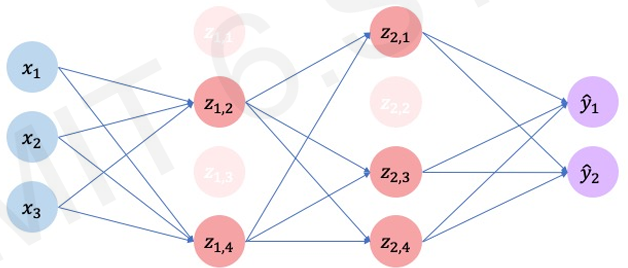
\includegraphics[width=\textwidth]{figures/regularization_dropout.PNG}
        % \caption{ML Production}
        % \label{fig:ML_Production}
    \end{minipage}
\end{center}
\vspace{-3pt}


$\bullet$ \textbf{Underfitting} or \textbf{High bias} means that the model is not able to capture (or learn) the trend (or pattern) in the data.

$\bullet$ \textbf{Overfitting} or \textbf{High variance} means that the model learns too much from the available data but does not generalize well enough to predict on \textbf{new data}.


\vspace{-3pt}
\begin{center}
    \begin{minipage}{0.8\linewidth}
        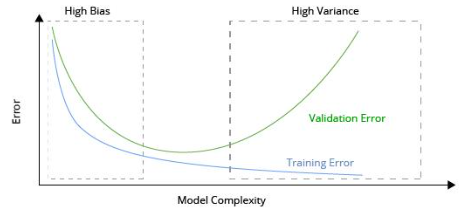
\includegraphics[width=\textwidth]{figures/Tradeoff_Learning_Curves.PNG}
        % \caption{ML Production}
        % \label{fig:ML_Production}
    \end{minipage}
\end{center}
\vspace{-3pt}

$\rightarrow$ The \textbf{training loss} goes down over time, achieving low error values
$\rightarrow$ The \textbf{validation loss} goes down until a turning point is found, and it starts going up again. That \textbf{point} represents the \textbf{beginning} of \textbf{overfitting}. Therefore, \textbf{The training process should be stopped when the validation error trend changes from descending to ascending}.


\vspace{-3pt}
\begin{center}
    \begin{minipage}{\linewidth}
        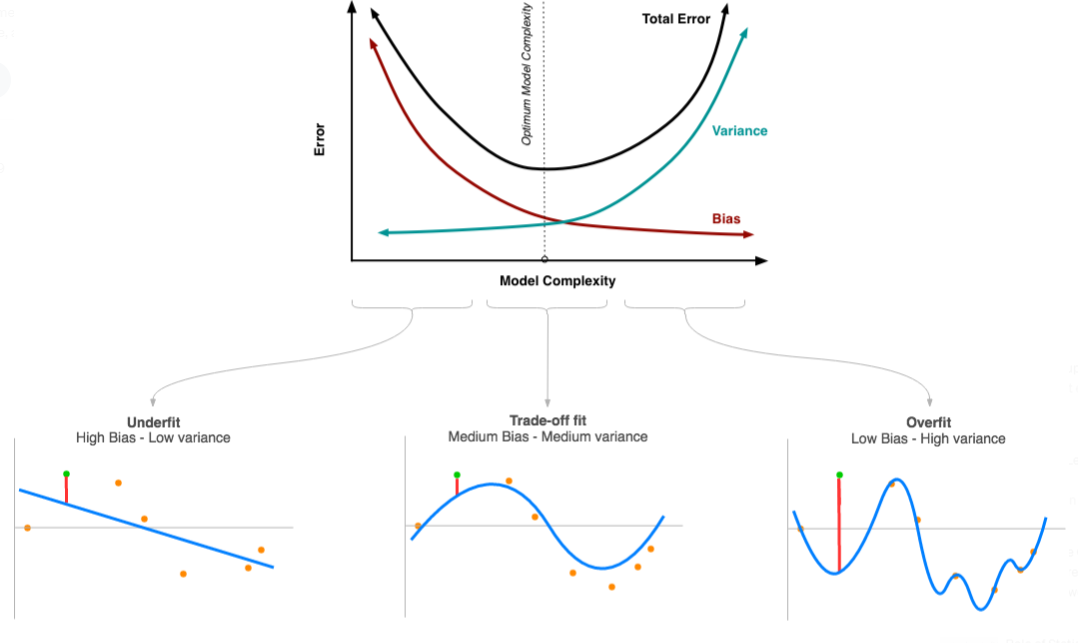
\includegraphics[width=\textwidth]{figures/bias_variance_overfitting_underfitting.PNG}
        % \caption{ML Production}
        % \label{fig:ML_Production}
    \end{minipage}
\end{center}
\vspace{-6pt}


\begin{center}
    \begin{minipage}{0.9\linewidth}
        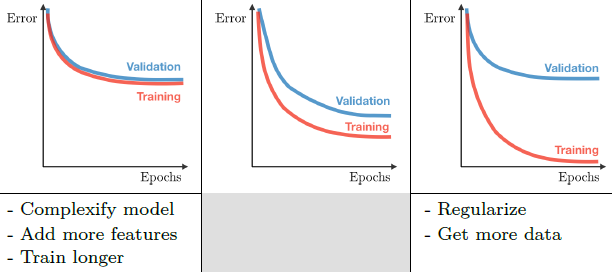
\includegraphics[width=\textwidth]{figures/bias_variance_overfitting_underfitting_LearningCurves.PNG}
        % \caption{ML Production}
        % \label{fig:ML_Production}
    \end{minipage}
\end{center}








$\bullet$ Training loss vs. Validation loss:
\vspace{-3pt}
\begin{center}
    \begin{minipage}{0.60\linewidth}
        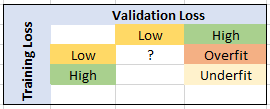
\includegraphics[width=\textwidth]{figures/Training_Validation_Loss.PNG}
        % \caption{ML Production}
        % \label{fig:ML_Production}
    \end{minipage}
\end{center}

\vspace{-3pt}

$\rightarrow$ \textbf{Epochs:} One Epoch is when an ENTIRE dataset is passed forward and backward through the neural network only ONCE.

$\rightarrow$ \textbf{Batch:} You can’t pass the entire dataset into the neural net at once. So, you divide dataset into No. of Batches or sets or parts.

$\rightarrow$ \textbf{Iterations} is the No. of Batches needed to complete One Epoch.

\textbf{Question}: If total number of samples in a dataset is 1000 and batch size is 10, how many iterations will be there in one epoch. \textbf{\textcolor{blue}{Ans}}: \textbf{100}

\vspace{3pt}
$\bullet$ \textbf{How would you identify if your model is overfitting?}
By analyzing the \textbf{learning curves}, you should be able to spot whether the model is underfitting or overfitting. The $y$-axis is some metric of learning (ex:, classification accuracy) and the $x$-axis is experience (time or No. of iteration).


\vspace{3pt}
$\bullet$ \textcolor{teal}{\textbf{What is cross-validation? Why it's important?}} \\
Cross-validation evaluates a model's performance. \\
$\rightarrow$ The idea is to divide the dataset into $k$ subsets or "folds", train the model on $k-1$ of these folds, and test on the remaining fold to ensure that the model generalizes well to unseen data. \\
$\rightarrow$ After evaluating on all k folds, performance metrics are averaged for a robust estimate of the model's effectiveness. \\
$\rightarrow$ \textbf{K-Fold Cross-Validation}: The data is divided into k equally-sized folds. \\
$\rightarrow$ \textbf{Stratified K-Fold}: Similar to K-Fold, but it maintains the proportion of classes in each fold, making it ideal for imbalanced datasets. \\
$\rightarrow$ \textbf{Leave-One-Out Cross-Validation (LOOCV)}: A special case where k equals the number of data points, so each fold contains just one data point.




\subsubsection{Unrepresentative Training Dataset} {\color{teal}\hrule height 0.5pt} \smallskip

When the data available during training is not enough to capture the model, relative to the validation dataset.

\vspace{-3mm}
\begin{center}
    \begin{minipage}{0.5\linewidth}
        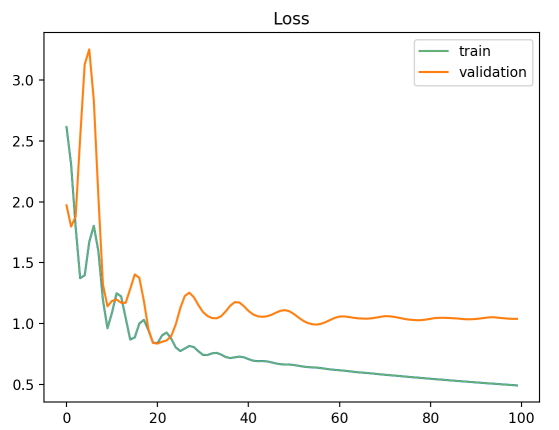
\includegraphics[width=\textwidth]{figures/Unrepresentative_Training_Dataset.PNG}
        % \caption{ML Production}
        % \label{fig:ML_Production}
        % \end{minipage}
    \end{minipage} 
\end{center}
\vspace{-3mm}


% \begin{wrapfigure}{l}{0.7\linewidth}
% 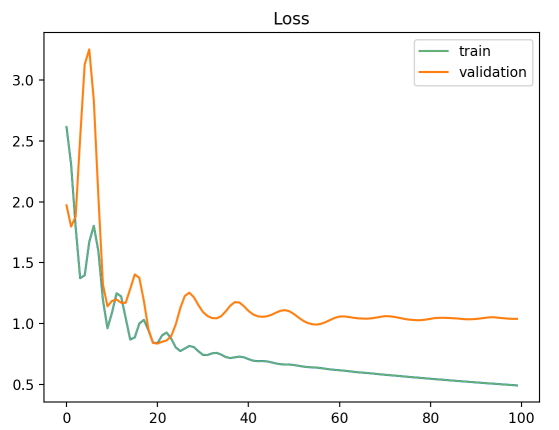
\includegraphics[width=\linewidth]{figures/Unrepresentative_Training_Dataset.PNG}
% \caption{This is the Overleaf logo}
% \end{wrapfigure}




The train and validation curves are improving, but there’s a big gap between them, which means they operate like datasets from different distributions.

\subsubsection{Unrepresentative Validation Dataset} {\color{teal}\hrule height 0.5pt} \smallskip

\begin{center}
    \begin{minipage}{0.5\linewidth}
        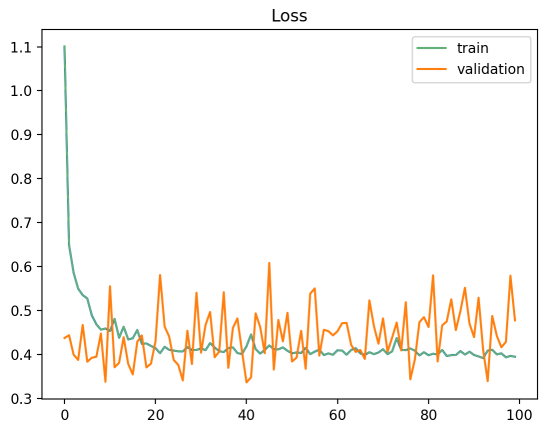
\includegraphics[width=\textwidth]{figures/First_scenario_Unrepresentative_Validation_Dataset.PNG}
        % \caption{ML Production}
        % \label{fig:ML_Production}
        % \end{minipage}
    \end{minipage} 
\end{center}
\vspace{-3mm}

As we can see, the training curve looks ok, but the validation function moves noisily around the training curve.
It could be the case that validation data is scarce and not very representative of the training data, so the model struggles to model these examples.

\vspace{-3mm}
\begin{center}
    \begin{minipage}{0.5\linewidth}
        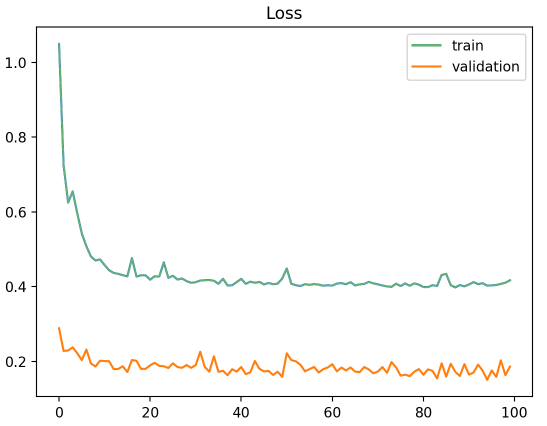
\includegraphics[width=\textwidth]{figures/Second_scenario_Unrepresentative_Validation_Dataset.PNG}
        % \caption{ML Production}
        % \label{fig:ML_Production}
        % \end{minipage}
    \end{minipage} 
\end{center}
\vspace{-3mm}
 
Here, the validation loss is much better than the training one, which reflects the validation dataset is easier to predict than the training dataset. An explanation could be the validation data is scarce but widely represented by the training dataset, so the model performs extremely well on these few examples.



% \vspace*{\fill}

% \columnbreak


\subsection{Data Science General} {\color{teal}\hrule height 0.5pt} \smallskip

\subsubsection{Inference vs. Classification} {\color{teal}\hrule height 0.5pt} \smallskip


$\rightarrow$ \textbf{Inference}: Given two groups, what is the differences between these groups? t-tests, paired t-test etc. \\
$\rightarrow$ \textbf{Classification}: Given a new animal, find whether new animal is cat or dog? \\



\subsubsection{Prediction and Inference} {\color{teal}\hrule height 0.5pt} \smallskip

$\rightarrow$ \textbf{Prediction} uses a model to predict future observations.\\
\hspace{5pt} - Model does not need to be valid \\
\hspace{5pt} - Evaluation does need to be valid \\
\hspace{5pt} - Quality \& strength: accuracy of predicting unseen data\\

\vspace{3pt}

$\rightarrow$ \textbf{Inference} uses the model’s structure and parameters to learn or understand an underlying phenomenon.\\
\hspace{5pt} - Validity depends on assumptions\\
\hspace{5pt} - Quality \& strength: $R^{2}$, p-value, assumption checks, coefficients\\







\subsubsection{Preventing Data Leakage} {\color{teal}\hrule height 0.5pt} \smallskip

\begin{itemize} [leftmargin=0.5cm]
    \item \textbf{Proper Data Splitting}: Split data into training, validation, and test sets \textbf{before} performing any data preprocessing. For time series, split data chronologically.
    \vspace{-3pt}
    \item \textbf{Transformation fit on Training Data Only}: Ensure that transformations (e.g., scaling, encoding) are fit only on the training data and then applied to both training and test data
    \item \textbf{Feature Selection}: Ensure that features used for training are available at the time of prediction. For time series data, create lag features that use only past information.
    \vspace{-3pt}
    % \item \textbf{Target Leakage}: Ensure that features used in training are available at the time of prediction and do not contain information derived from the target variable.
    % \vspace{-3pt}
    \item \textbf{Data Augmentation}: Apply augmentation techniques only to the training set. 
\end{itemize}



\subsubsection{Handle missing or corrupted data in a dataset} {\color{teal}\hrule height 0.5pt} \smallskip

\begin{itemize} [leftmargin=0.5cm]
    \item \textbf{Remove Missing Data}: If only a small number of \textbf{rows} have missing values, or If an entire \textbf{column} has a large percentage of missing values
    \vspace{-3pt}
    \item \textbf{Impute Missing Data}: Mean/Median/Mode Imputation, Imputation Using Algorithms like Forward/Backward Fill/ Interpolate for time series data
    \item \textbf{Use Algorithms That Handle Missing Data}: Decision trees, Random forests
    \vspace{-3pt}
    \item \textbf{Replace Corrupted Data}: Identify Outliers using statistical methods (like z-scores or IQR), Apply manual inspection and correction of corrupted values based on external sources or domain expertise.
    \vspace{-3pt}
    \item \textbf{Data Augmentation}: To create synthetic data based on existing patterns
\end{itemize}



\subsubsection{Notes} {\color{teal}\hrule height 0.5pt} \smallskip

$\rightarrow$ \textbf{Ablation}: An ablation study is turning off components of a model (e.g. features or sub-models) one at a time, to see how much each contributes to the model's performance. \\

\subsubsection{ETL - Extract Transform Load} {\color{teal}\hrule height 0.5pt} \smallskip

An ETL workflow is crucial for consolidating and preparing data for analysis and reporting, ensuring accuracy, consistency, and availability for better decision-making.


\begin{enumerate}[leftmargin=0.37cm]
    \item \textcolor{blue}{\textbf{Extract Phase}:} Retrieve raw data from sources like databases, files, or APIs using SQL queries, scripts, or connectors. Extract only the new or updated data since the last extraction to optimize performance and reduce load.  \\
   


    \item \textcolor{blue}{\textbf{Transform Phase}:}  Clean, integrate, and format data, applying business rules and calculations. Validate transformations and ensure data quality using tools like Python, SQL, or Apache Spark. \\


    \item \textcolor{blue}{\textbf{Load Phase}:}  Insert transformed data into the target system, ensuring correct schema, bulk loading for efficiency, and optimizing with indexing and partitioning. \\
   
\end{enumerate}

\vspace{5pt}
\textcolor{purple}{\textbf{ETL Workflow Automation}} \\
Automation Tools:  \\
$\rightarrow$ Apache Airflow: For workflow scheduling and orchestration.\\
$\rightarrow$ AWS Glue: Managed ETL service on AWS.\\
$\rightarrow$ Apache NiFi: For data flow automation.







\vspace*{\fill}










\subsection{Model Evaluation} {\color{teal}\hrule height 0.5pt} \smallskip

\subsubsection{Classification Problems} {\color{teal}\hrule height 0.5pt} \smallskip

\textbf{{\textcolor{purple}{Confusion Matrix}}} \\

\textbf{Type I error:} The null hypothesis $H_{0}$ is \textbf{rejected} when it is \textbf{true}. \\

\textbf{Type II error:} The null hypothesis $H_{0}$ is \textbf{not rejected} when it is \textbf{false}.

$\rightarrow$ \textbf{False negative} (\textbf{Type I error}) — incorrectly decide \textbf{no} \\
$\rightarrow$ \textbf{False positive} (\textbf{Type II error}) — incorrectly decide \textbf{yes} \\


\begin{center}
    \begin{minipage}{0.70\linewidth}
        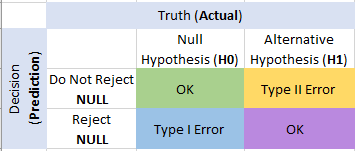
\includegraphics[width=\textwidth]{figures/Confusion_Matrix_1.PNG}
    \end{minipage}
\end{center}

\vspace{3pt}
\textbf{Ex:} We assume the null hypothesis $H_{0}$  is true. \\
$\rightarrow$ $H_{0}$: Person is not guilty  \\
$\rightarrow$ $H_{1}$: Person is guilty  \\


\begin{center}
    \begin{minipage}{\linewidth}
        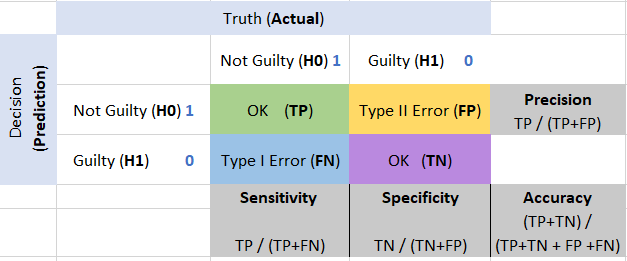
\includegraphics[width=\textwidth]{figures/Confusion_Matrix_2.PNG}
    \end{minipage}
\end{center}

\begin{center}
    \begin{minipage}{0.56\linewidth}
        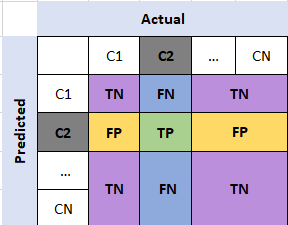
\includegraphics[width=\textwidth]{figures/confusion_matrix_multi_class.PNG}
    \end{minipage}
\end{center}



\begin{enumerate}
    \item \textbf{Accuracy: } $\boxed{\frac{TP + TN}{TP + TN + FP + FN}}$ \\
    $\rightarrow$ Ratio of \textbf{correct predictions} over \textbf{total predictions}. \\
    \textbf{Estimate} of $\boxed{P[D=Y]}$,  probability of decision is equal to outcome.
    \vspace{-3pt}
    \item \textbf{Recall} or \textbf{Sensitivity} or \textbf{True positive rate}: $\boxed{\frac{TP}{TP+FN}}$.  \underline{Completness} of model $\rightarrow$ Out of \textbf{total actual positive (1) values}, how often the classifier is correct. \\
    \textbf{Probability}: $\boxed{P[D=1 | Y=1]}$ \\
    \textbf{\textcolor{blue}{Example: }} "\underline{\textbf{Fradulent transaction detector}}" or "\underline{\textbf{Person Cancer}}" $\rightarrow$ +ve (1) is "fraud": Optimize for sensitivity because false positive (\textbf{FP} normal transactions that are flagged as possible fraud) are more acceptable than false negative (\textbf{FN} fradulent transactions that are not detected) 
    \vspace{-2pt}

    \item \textbf{Precision}: $\boxed{\frac{TP}{TP+FP}}$ \\
    \underline{Exactness } of model. $\rightarrow$ Out of \textbf{total predicted positive (1) values}, how often classifier is correct. \\ \textbf{Probability}: $\boxed{P[Y=1 | D=1]}$, If our model says positive, how likely it is correct in that judgement.\\
    \textbf{\textcolor{blue}{Example: }} "\underline{\textbf{Spam Filter}}" +ve (1) class is spam $\rightarrow$ Optimize for precision or, specificity because false negatives (\textbf{FN} spam goes to the inbox) are more acceptable than false positive (\textbf{FP} non-spam is caught by the spam filter).
    \textbf{\textcolor{blue}{Example: }} "\underline{\textbf{Hotel booking canceled}}" +ve (1) class is isCanceled $\rightarrow$ Optimize for precision or, specificity because false negatives (\textbf{FN} isCanceled labeled as "not canceled" 0) are more acceptable than false positive (\textbf{FP} isnotCanceled labeled as "canceled" 1).
    \vspace{-2pt}

    \item \textbf{F1-Score } = $\boxed{2 \times \frac{\text{Precision} \times \text{Recall}}{\text{Precision} + \text{Recall}}}$  \\
    False positive (FP) and False negative (FN) are equally important.
    \vspace{-2pt}

    \item \textbf{False Positive Rate}: \(\boxed{\frac{FP}{TN+FP}} \) \\
    Fraction of \textbf{negatives} wrongly classified positive. \\  \textbf{Probability}: $\boxed{P[D=1 | Y=0]}$
    \vspace{-2pt}

    \item \textbf{False Negative Rate}: \(\boxed{\frac{FN}{TP+FN}} \) = 1 - Recall  \\
    Fraction of \textbf{positives} wrongly classified negative.  \\
    \textbf{Probability}: $\boxed{P[D=0 | Y=1]}$
    \vspace{-2pt}
    
    \item \textbf{Specificity}: \(\boxed{\frac{TN}{TN+FP}} \) = 1-FPR  \\
    Fraction of \textbf{negatives} rightly classified negative.  \\\textbf{Probability}: $\boxed{P[D=0 | Y=0]}$
\end{enumerate}



$\bullet$ \textbf{ROC}-curve: The curve illustrates the trade-off between (TPR) true positive rate \textbf{(sensitivity or recall)} and the (FPR) false positive rate using classification thresholds $\alpha$.


$\rightarrow$ Lowering the classification threshold classifies more items as positive, thus increasing both False Positives and True Positives.

\vspace{-3pt}

\begin{center}
    \begin{minipage}{0.75\linewidth}
        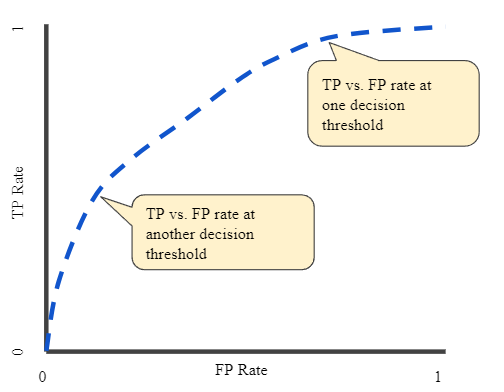
\includegraphics[width=\textwidth]{figures/ROC_curve.PNG}
    \end{minipage}
\end{center}

\vspace{-5pt}

\textbf{Note:} We can think of the plot as the fraction of \textbf{correct predictions for the positive class} (y-axis) versus the fraction of \textbf{errors for the negative class} (x-axis).

\vspace{2pt}

\textbf{\textcolor{blue}{How to choose threshold for the logistic regression?}}
The choice of a threshold depends on the importance of TPR and FPR classification problem. If there is no external concern about low TPR or high FPR, one option is to weight them equally by choosing the threshold that maximizes TPR$-$FPR.
\begin{lstlisting}[language=Python, mathescape=true, frame=single]
# Get predicted probabilities
y_prob = model.predict_proba(X_test)[:, 1] 
# Calculate ROC curve
fpr, tpr, thresholds = roc_curve(y_test, y_prob)
# Optimal threshold using Youden's J stat.
youden_index = tpr - fpr
optimal = thresholds[np.argmax(youden_index)]
\end{lstlisting}


\vspace{3pt}

$\bullet$ Area Under the ROC Curve \textbf{AUC}: To compute the points in an ROC curve, an efficient, sorting-based algorithm called AUC. AUC ranges in value from 0 to 1. Area Under the Curve measures how likely the model differentiates positives and negatives (perfect AUC = 1, basline = 0.5) 

% \vspace{-5pt}

% \begin{center}
%     \begin{minipage}{0.55\linewidth}
%         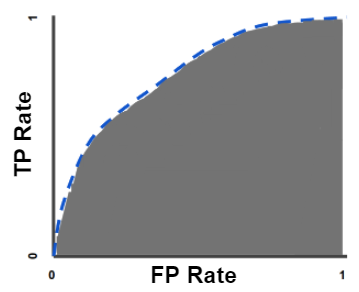
\includegraphics[width=\textwidth]{figures/AUC_ROC.PNG}
%     \end{minipage}
% \end{center}
% \vspace{-5pt}




\vspace{3pt}
$\bullet$ \textbf{Precision-Recall} curve: Focuses on the correct prediction of the \textbf{minority} class, useful when data is \textbf{imbalanced}. Plot precision at different thresholds.

\vspace{-5pt}
\begin{center}
    \begin{minipage}{0.75\linewidth}
        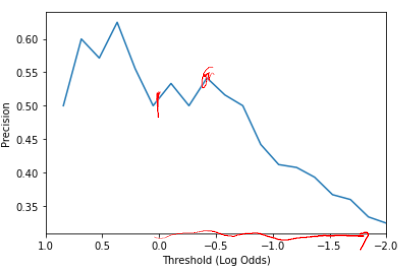
\includegraphics[width=\textwidth]{figures/Precision_Curve.PNG}
    \end{minipage}
\end{center}


\vspace{-5pt}




\subsubsection{Regression Problems} {\color{teal}\hrule height 0.5pt} \smallskip

\begin{enumerate}
    \item \textbf{Mean Squared Error: } \(\boxed{\text{MSE} = \frac{1}{n} \sum_{i}(y_{i} - \hat{y_{i}})^{2}} \)
    
    \item \textbf{Root Mean Squared Error: } \(\boxed{\text{RMSE} = \sqrt{\frac{\sum^{N}_{i=1} (y_{i} - \hat{y_{i}})^{2}}{N}}}\)
    
    \item \textbf{Mean Absolute Error: } \(\boxed{\text{MAE} = \frac{1}{n} \sum_{i} |y_{i}-\hat{y_{i}}| }\)
    
    \item \textbf{Sum of Squared Error:} \(\boxed{\text{SSE} = \sum_{i} (y_{i} - \hat{y_{i}})^{2}}  \) 
    
    \item \textbf{Total Sum of Squares:} \(\boxed{\text{SST} = \sum_{i} (y_{i} - \bar{y_{i}})^{2}}\)
    
    \item \textbf{$R^{2}$ Error : }  
    \vspace{-3pt}
    \[\boxed{R^{2} = 1 - \frac{\text{MSE (model)}}{\text{MSE(baseline)}}} \hspace{15pt} \boxed{R^{2} = 1 - \frac{\text{SSE}}{\text{SST}}} \] 
    
    
    \item \textbf{Adjusted} $R^{2}$ :
    \vspace{-3pt}
    \[\boxed{R^{2}_{a} =  1 - \left[ \left( \frac{n-1}{n-k-1} \right) (1-R^{2})   \right]} \] 
\end{enumerate}

\subsubsection{Variance, \texorpdfstring{\(R^{2}\)}, and the Sum of Squares}  {\color{teal}\hrule height 0.5pt} \smallskip

$\bullet$ The \textbf{total sum of squares}: $\text{SS}_{\text{total}}$ = \(\sum_{i} (y_{i} - \bar{y})^{2} \) \\

$\bullet$ This scales with variance: var($Y$) = \( \frac{1}{n} \sum_{i} (y_{i} - \bar{y})^{2} \) \\

$\bullet$ The \textbf{regression} sum of squares: \\
$\text{SS}_{\text{regression}}$ = \(\sum_{i} \hat{(y_{i}} - \bar{y})^{2} \), $\rightarrow$ nVar(predictions)

$\bullet$ The \textbf{residual} sum of squares (squared errro): \\ 
$\text{SS}_{\text{residual}}$ = \(\sum_{i} (y_{i} - \hat{y_{i}})^{2} \), $\rightarrow$ nVar($\epsilon$) \\

\vspace{2pt}
\textbf{\textcolor{blue}{Note: }} \(\bar{\epsilon} = 0, E[\hat{y}] = \bar{y} \)
\vspace{-3pt}
\[\text{SS}_{\text{total}} = \text{SS}_{\text{regression}} + \text{SS}_{\text{residual}} \]
\vspace{-3pt}
\[R^{2} = 1 - \frac{\text{SS}_{\text{residual}}}{\text{SS}_{\text{total}}} = \frac{\text{SS}_{\text{regression}}}{\text{SS}_{\text{total}}} = \frac{nVar(\text{preds})}{nVar(Y)} = \frac{Var(\text{preds})}{Var(Y)}\]
\vspace{-3pt}

$\rightarrow$  \textbf{Explained Variance}: $R^{2}$ quantifies how much of the variability in the outcome (\textbf{dependent}) variable can be explained by the predictor (\textbf{independent}) variables. 


$\rightarrow$ \textbf{Goodness of Fit}: A higher $R^{2}$
value generally suggests a better fit of the model to the data, meaning the model's predictions are closer to the actual values. 

$\rightarrow$ An $R^{2}$ of 1 indicates a perfect fit, where the model explains all the variability, while an $R^{2}$ of 0 indicates that the model explains none of the variability.

$\rightarrow$ \textbf{$R^{2}$ is not valid for nonlinear models} as 
\vspace{-2pt}
\[\boxed{\text{SS}_{\text{residual}} + \text{SS}_{\text{error}} \neq \text{SS}_{\text{total}}}\]
\vspace{-3pt}

$\rightarrow$ \textbf{Drawback}: R-squared will always increase when a new predictor variable is added to the regression model, that's why \textbf{adjusted} $R^{2}$ used

% \begin{minipage}{\linewidth}
% % \begin{figure}[h!]
%     \centering
%     % \begin{minipage}[b]{\textwidth}
%     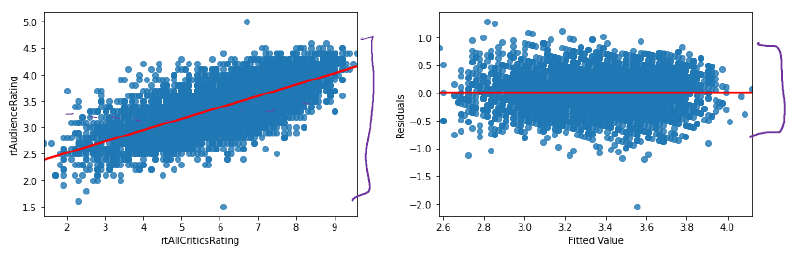
\includegraphics[width=\textwidth]{figures/Residual_variance.PNG}
%     % \caption{ML Production}
%     % \label{fig:ML_Production}
%     % \end{minipage}
% % \end{figure}
% \end{minipage}








% \columnbreak



\subsection{Optimization} {\color{teal}\hrule height 0.5pt} \smallskip

Almost every machine learning method has an optimization algorithm at its core. \\
$\rightarrow$ \textbf{Hypothesis :} The hypothesis $h_{\theta}$ is the model that we choose. For a given input data $x^{(i)}$ the model prediction output is $\boxed{h_{\theta}(x^{(i)})}$. 

\vspace{3pt}

$\rightarrow$ \textbf{Loss function : } 
\(\boxed{L:(\hat{y},y)  \in  R \times Y \longmapsto  L(\hat{y},y) \in R} \) that takes as inputs the \textbf{predicted} $\hat{y}$, the \textbf{actual}  $y$, and outputs how different they are. \\
In another way, The \textbf{loss function} computes the \textbf{distance} or \textbf{difference} between the \textbf{predicted} output $\hat{y}$ of the algorithm and the \textbf{actual} output $y$. 

\vspace{3pt}
The common loss functions are summed up in the table below:
\vspace{-5pt}
\begin{center}
    \begin{tabular}{c|c|c}
            \textbf{Least squared error} & \textbf{Logistic loss} & \textbf{Hinge loss} \\
            \hline
             $\frac{1}{2}(y-\hat{y})^{2}$ & $\text{log}\left(1+\text{exp}(-y\hat{y})\right)$ & $\text{max}(0, 1-y\hat{y})$  \\
            \hline 
            Linear Regression & Logistic Regression & SVM \\
            \hline
            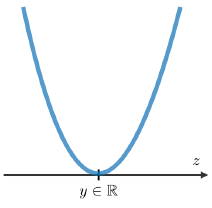
\includegraphics[scale = 0.4]{figures/least_squared_loss_func.PNG} &
            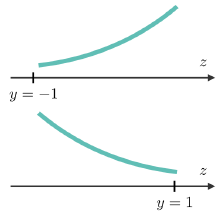
\includegraphics[scale = 0.4]{figures/logistic_loss_func.PNG} &
            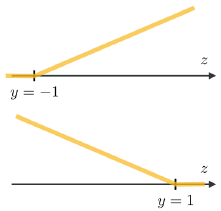
\includegraphics[scale = 0.4]{figures/hinge_loss_func.PNG}
    \end{tabular}
\end{center}



$\rightarrow$ \textbf{Cost function :} The cost function $J$ is commonly \textbf{used to know the performance of a model}, and is defined with the loss function $L$ as follows: 
\vspace{-3pt}
\[\boxed{J(\theta) = \sum^{m}_{i=1} L(h_{\theta}(x^{(i)}) , y^{(i)})} \]

$\bullet$ Cost function for \textbf{regression}: Mean Squared Error (MSE), Mean Absolute Error (MAE), Huber Loss, Log-Cosh Loss

$\bullet$ Cost function for \textbf{classification}: Binary Cross-Entropy Loss, Categorical Cross-Entropy Loss, Sparse Categorical Cross-Entropy Loss, Hinge Loss, Squared Hinge Loss.



\subsubsection{Convex \& Non-convex} {\color{teal}\hrule height 0.5pt} \smallskip

A \textbf{convex} function is one where a line drawn between any two points on the graph lies on or above the graph. It has \textbf{one minimum}. A \textbf{non-convex} function is one where a line drawn between any two points on the graph may intersect other points on the graph. It characterized as "wavy"\\

$\rightarrow$ When a \textbf{cost function is non-convex}, it means that there is a likelihood that the function may find \textbf{local minima} instead of the \textbf{global minimum}, which is typically undesired in machine learning models from an optimization perspective.

\subsubsection{General Optimization Steps} {\color{teal}\hrule height 0.5pt} \smallskip
1. Understand data (features and outcome variables) $\rightarrow$
2. Define loss (or gain/utility) function $\rightarrow$
3. Define predictive model $\rightarrow$
4. Search for parameters that minimize the loss function

\subsubsection{Gradient Descent} {\color{teal}\hrule height 0.5pt} \smallskip

Gradient Descent is used to \textbf{find the coefficients} of $f$ that
\textbf{minimizes a cost function}. \\
$\rightarrow$ \textbf{Time Complexity}: \(O(n \cdot m) \) $\rightarrow$ $n$ is no. of data points, $m$ no. of features. If you run for $k$ iterations the total complexity becomes   \(O(k \cdot n \cdot m) \)

$\rightarrow$ It minimizes the average loss by moving iteratively in the direction of steepest descent, controlled by the learning rate $\gamma$ (step size). 

\textbf{Procedure: }
\begin{enumerate}
    \item Intialization  \hspace{14pt} \(\theta = 0\) \textcolor{blue}{(coefficients to 0 or random)}
    \item Calculate cost  \hspace{5pt} \(J(\theta) = \text{evaluate\big($f$(coefficients)}\big)\)
    \item Gradient of cost \hspace{-2pt} $\frac{\partial}{\partial \theta_{j}} J(\theta)$ \textcolor{blue}{we knows the uphill direction} 
    \item Update coeff \hspace{12pt} $\theta_{j} = \theta_{j} - \alpha \frac{\partial}{\partial \theta_{j}} J(\theta)$ \textcolor{blue}{we go downhill}
\end{enumerate}
The cost updating process is repeated until convergence (minimum found). 
\vspace{-7pt}
\begin{center}
    \begin{minipage}{0.75\linewidth}
        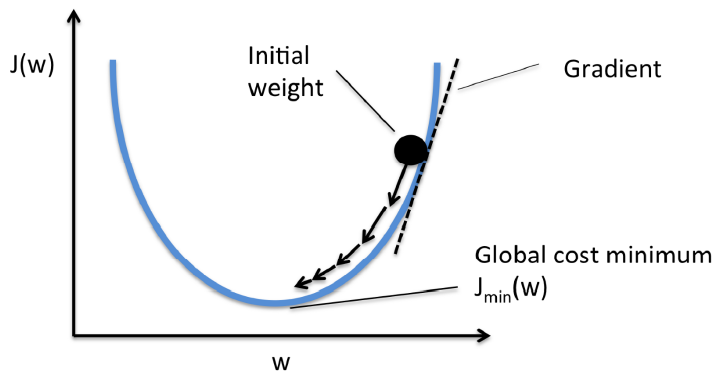
\includegraphics[width=\textwidth]{figures/gradient_decent.PNG}
    \end{minipage}    
\end{center}
\vspace{-5pt}

\textbf{Tips : }
For effective gradient descent, select an optimal learning rate, scale features, initialize parameters wisely, utilize mini-batch processing, monitor convergence, experiment with various optimizers, apply regularization techniques, avoid local minima, visualize loss trends, and tune hyperparameters diligently.

\vspace{3pt}

$\bullet$ \textbf{Stochastic Gradient Descent} uses a single point to compute gradients, leading to smoother convergence and faster compute speeds. \\
$\rightarrow$ \textbf{Time Complexity}: \(O(k \cdot m) \) $\rightarrow$ $m$ is no. of features. In each iteration, SGD computes the gradient using only one data point, leading to \(O(k 
 \cdot m)\) for $m$ features. 



$\bullet$ \textbf{Mini-batch Gradient Descent} trains on small subsets of the data, striking a balance between the approaches.
$\rightarrow$ \textbf{Time Complexity}: \(O(k \cdot b \cdot m) \) 






\subsubsection{Ordinary Least Squares} {\color{teal}\hrule height 0.5pt} \smallskip

\textbf{General Linear Regression Model:} \(\boxed{\hat{y} = \beta_{0} + \sum_{j}\beta_{j}x_{j} + \epsilon} \)

Here, $\beta_{j}$ is the $j$-th coefficient and $x_{j}$ is the $j$-th feature.

\vspace{3pt}

\textbf{Ordinary Least Squares} - find $\Vec{\beta}$ that minimizes \textbf{squared error}:

\[ \boxed{ \underset{\vec{\beta}} {\arg\min} \sum_{i} \left(y_{i} - \hat{y_{i}}  \right)^2} \]

\begin{center}
    \begin{minipage}{0.75\linewidth}
    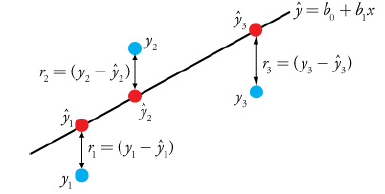
\includegraphics[width=\textwidth]{figures/ordinary_least_square.PNG}
\end{minipage}
\end{center}


\textbf{Goal: }least-squares solution to : \(\boxed{X \Vec{\beta} = \hat{y} }\) \\
\textbf{Solution: } solve the normal equations:
\vspace{-2pt}
\[
    X^{T} X \Vec{\beta} = X^{T} \hat{y} 
    \hspace{10pt}  \rightarrow \vec{\beta}  = (X^{T}X)^{-1} X^{T} \hat{y} 
\]
\vspace{-7pt}
\[ \boxed{L(\Vec{\beta} \;| \Vec{X}, \hat{y} )} \]








$\rightarrow$ Least squares generalizes into \textbf{minimizing loss functions}. \\
$\rightarrow$ This is the heart of machine learning, particularly supervised learning.



\vspace{5pt}
\subsubsection {\textbf{Likelihood and Posterior}} {\color{teal}\hrule height 0.5pt} \smallskip
\[\mathcolor{orange}{P(\theta |\textbf{y})} = \frac{\mathcolor{green}{P(\textbf{y}|\theta)} \, \mathcolor{purple}{P(\theta)} }{P(\textbf{y})} \]
\vspace{-5pt}

• \mathcolor{Purple}{$P(\theta)$} is the \textcolor{Purple}{prior}
\\

• \mathcolor{Green}{$P(y | \theta)$} is the \textcolor{Green}{likelihood} – how likely is the data given params $\theta$ \\
• $P(y) = \int P(y | \theta) P(\theta) d\theta $ is a scaling factor (constant for fixed $y$) \\
• $\mathcolor{Orange}{P(\theta | y)}$ is the \textcolor{Orange}{posterior}.


• We’re maximizing likelihood (ML estimator) \\
• Can also maximize posterior (MAP estimator)\\
\hspace{7pt} - When prior is constant, they’re the same\\
\hspace{7pt} - With lots of data, they’re almost the same\\

$\rightarrow$ Logistic function is trained by
\textbf{maximizing the log likelihood} of the
training data given the model



\vspace{2pt}
\subsubsection{Maximum Likelihood Estimation (\textbf{MLE})} {\color{teal}\hrule height 0.5pt} \smallskip
In MLE, the goal is to estimate the parameters (or coefficients) of a probability distribution by finding the values that \textbf{maximize} the likelihood of the observed data.

\vspace{3pt}
$\bullet$ \textbf{Likelihood Function}: The likelihood function measures the probability of the observed data given the parameters. It helps to evaluate how well different parameters explain the observed data.
For a dataset \(X = \{x_{1}, x_{2}, ... {x_n} \}\), assumed to be i.i.d.and a parameter $\theta$, the likelihood \(L(\theta)\) is: 
\vspace{-3pt}
\[\boxed{L\left(\theta | X \right) = \prod^{n}_{i=1} f\left(x_{i}|\theta \right) \hspace{4pt} \rightarrow L\left(\theta | X \right) = P\left(X | \theta \right) =  \prod^{n}_{i=1} P\left(x_{i}|\theta \right) }   \]

$\bullet$\textbf{ Log-Likelihood}:
The natural log of $L(\theta)$ is then taken prior to calculating the maximum because multiplying probabilities can result in very small values and also log is a monotonically increasing function, maximizing the \textbf{log-likelihood} log $L(\theta)$ is equivalent to maximizing the likelihood:
\vspace{-3pt}
\[\boxed{\text{log} \hspace{2pt} L\left(\theta | X \right) = \text{log} \hspace{2pt} P\left(X | \theta \right) =  \prod^{n}_{i=1} \text{log} \hspace{2pt} P\left(x_{i}|\theta \right) }   \]




$\rightarrow$ MLE is used to find the estimators that \textbf{minimized the likelihood function:} 
\(\mathcal{L}(\theta|x) = f_{\theta}(x) \) \hspace{5pt} \textcolor{blue}{density function of the data distribution}



\vspace{3pt}



In case of \textbf{Logistic Regression}:
\vspace{-10pt}
\[P\left(Y=1 | X=x \right) = \hat{y} = \text{logistic} \left(\beta_{0} + \sum_{j} \beta_{j}x_{j} \right)  \]
\vspace{-12pt}

The model computes \textbf{probability of yes}.\\
$\rightarrow$ What if we want $P(Y=y_{i})$, regardless of whether $y_{i}$ is 1 or 0? \\
\vspace{-5pt}
\[P \left(Y=y_{i} | X=x_{i} \right) = \hat{y_{i}}^{y_{i}} \left(1- \hat{y_{i}}\right)^{1-y_{i}}  \]

\begin{itemize}
    \item $\hat{y}_{i}$ is model's estimate of $P(Y=1|X=x_{i})$
    \item $y_{i} \in \{0,1 \}$ is outcome
    \item $\hat{y}_{i}^{y_{i}}$ is $\hat{y}_{i}$ if $y_{i} = 1$, and $1$ if $y_{i} = 0$ 
\end{itemize}

\textbf{Conditioning on Parameters} \\
Fuller definition -  condition on parameters $\vec{\beta}$ and write function: 
\vspace{-2pt}
\[P(Y=1|x, \vec{\beta}) = \hat{y} = m(x, \vec{\beta}) = \text{logistic(...)}\]

\vspace{3pt}
\textbf{Likelihood Function} \\


Given data \(\textbf{X} = \langle x_{1}, ..., x_{n}\rangle, \hspace{2pt}  \textbf{y} = \langle y_{1}, ... , y_{n} \rangle \) and parameters $\hat{\beta}$
\vspace{-3pt}

\[\text{Likelihood} (\textbf{y}, \textbf{X}, \vec{\beta}) = P(\textbf{y},\textbf{X}|\vec{\beta}) = \prod_{i} P(y_{i}|x_{i}, \vec{\beta}) \]


\vspace{-3pt}

By joint conditional probability, 
\vspace{-2pt}
\[ P(\textbf{y},\textbf{X} | \vec{\beta}) =  P(\textbf{X}|\vec{\beta}) \cdot P(\textbf{y} | \textbf{X}, \vec{\beta}) \]

But \textbf{X} is independent of params, so \(P(\textbf{X}|\vec{\beta}) = P(\textbf{X}) \). And \textbf{X} is fixed, so \(P(\textbf{X}) \) is an (unknown) constant.

\vspace{-5pt}

\[\text{log Likelihood}(\textbf{y},\textbf{X}, \vec{\beta}) = \text{log} \, P(\textbf{X}) \prod_{i} P\left( y_{i}|x_{i}, \vec{\beta} \right) \]
\vspace{-5pt}
\[= \text{log} \, P(\textbf{X})  + \sum_{i} \text{log} \, P \left( y_{i}|x_{i}, \vec{\beta} \right) \] 

\vspace{3pt}
\textbf{Maximum Likelihood Estimator}
\[ \underset{\vec{\beta}} {\arg\max} \sum_{i} \text{log} P\left(y_{i} | x_{i}, \vec{\beta} \right) \]

\vspace{-5pt}

\[P \left(Y=y_{i} | X=x_{i} \right) = \hat{y_{i}}^{y_{i}} \left(1- \hat{y_{i}}\right)^{1-y_{i}}  \]

\vspace{-10pt}

\[\text{log} P \left(Y=y_{i} | X=x_{i} \right) = y_{i} \; \text{log}\,  \hat{y_{i}} +  (1-y_{i}) \, \text{log}\left(1- \hat{y_{i}}\right)  \]

Model log likelihood is sum over training data. Applicable to \textbf{any} model where \(\hat{y} = P(Y=1 |x) \) 


\subsubsection{Bayesian Estimation - Maximum a Posterior (\textbf{MAP})} {\color{teal}\hrule height 0.5pt} \smallskip
\textbf{MAP} estimation seeks to find the parameters $\theta$ that maximize the posterior distribution, which assumes a "prior distribution \( P(\theta) \)"


\vspace{-3pt}
\[\boxed{\hat{\theta}_{MAP} = \underset{\theta}{\text{argmax}} \ P(\theta | X) = \underset{\theta}{\text{argmax}} \ \frac{P(X | \theta) P(\theta)}{P(X)} } \]
Since \( P(X) \) does not depend on \( \theta \),
\vspace{-3pt}
\[\boxed{\hat{\theta}_{MAP} \approx \underset{\theta}{\text{argmax}} \ P(X | \theta) P(\theta)}\]



In logistic regression, MAP can be applied by introducing a prior on the model parameters \( P(\theta) \)


% % \vspace*{\fill}

% % \columnbreak

\vspace{10pt}


\subsection{Linear Algorithms} {\color{teal}\hrule height 1pt} \smallskip


\subsubsection{Regression} {\color{teal}\hrule height 0.5pt} \smallskip

$\rightarrow$ Regression predicts (or estimates) a continuous variable 

\vspace{2pt}


\textbf{Dependent} variable $Y$, \textbf{Independent} variable(s) $X$ \\
$\rightarrow$ compute estimate $\hat{y} \approx y$
\vspace{-5pt}
\[\hat{y_{i}} = \beta_{0} + \beta_{1}x_{i} \]
\vspace{-10pt}
\[ y_{i} = \hat{y_{i}} +  \epsilon_{i} \]
Here, $\beta_{0}$ is intercept, $\beta_{1}$ is slope and $\epsilon$ is residuals. The goal is to learn $\beta_{0}, \beta_{1}$ to minimize $\sum \epsilon^{2}_{i}$ (least squares)

% \textbf{\textcolor{blue}{Note:}} \textbf{coef - } strength of relationship, \textbf{$R^{2}$ - } frac. of variance explained \\
% Regression predicts one value with another. \\
% Lets us go beyond same-scale (paired t-test) to determine strength of relationship.








\vspace{5pt}
\textbf{Linearity}: A linear equation of $k+1$ variables is of the form:
\[\hat{y} = \beta_{0} + \beta_{1}x_{1} + \cdots + \beta_{k}x_{k} \]

It is the \textbf{sum} of \textbf{scalar multiples} of the individual variables - aline!



% \subsubsection{Purpose of Modelling}
% • Understand predictor/outcome relationships \\
% \hspace{10pt} Correlational, not causal (at least alone)\\
% • Predict future outcomes\\
% • Estimate hypothetical outcomes\\
% • Correct for effects for further analysis\\

\vspace{3pt}


$\rightarrow$ Linear models are remarkably capable of transforming many non-linear problems into linear.






\subsubsection{Linear Regression} {\color{teal}\hrule height 0.5pt} \smallskip

\[\hat{y_{i}} = \beta_{0} + \beta_{1} x_{i1} + \beta_{2} x_{i2} \cdots + \beta_{p} x_{ip} + \epsilon  \]

\vspace{-7pt}

\[\boxed{\hat{y_{i}} = \beta_{0} + \sum^{n}_{i=1}\sum^{p}_{j=1}\beta_{j}x_{ij}}\]
Here, $n$ is total no. of observation, $\hat{y}_{i}$ is dependent variable, $x_{ij}$ is explanatory variable of $j$-th features of the $i$-th observation.
$\beta_{0}$ is intercept or usually called \textbf{bias} coefficient. \\



\textbf{\underline{Assumptions}:} \\
$\rightarrow$  Linear models make \textbf{four} key assumptions necessary for inferential
validity. \\
• \textbf{Linearity} — outcome $y$ and predictor $X$ have linear relationship. \\
• \textbf{Independence} — observations are independent of each other\\
- Independent variables (features) are not highly correlated with each other $\rightarrow$ \textbf{Low multicollinearity} \\
• \textbf{Normal errors} — residuals are normally distributed - \textbf{check} with Q-Q plots.\textbf{ Violation} means line (in Q-Q plots) still fits but p-value and CIs are unreliable\\
• \textbf{Equal variance} — residuals have constant variance (called
homoskedasticity; violation is heteroskedasticity) - \textbf{check} scatterplot or regplot between residuals vs. fitted. \textbf{Violations} means model is failing to capture a systematic effect. $\rightarrow$  These violations are problem only for inference not for prediction



\begin{minipage}{\linewidth}
% \begin{figure}[h!]
    \centering
    % \begin{minipage}[b]{\textwidth}
    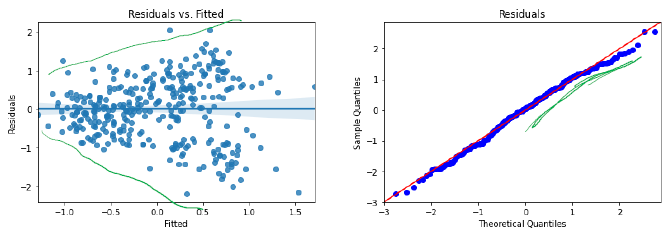
\includegraphics[width=\textwidth]{figures/Violation_EqualVariance_and_NormalErros.PNG}
    % \caption{ML Production}
    % \label{fig:ML_Production}
    % \end{minipage}
% \end{figure}
\end{minipage}





\vspace{3pt}
\textcolor{purple}{Variance Inflation Factor :} Measures the severity if multicollinearity $\rightarrow \boxed{\frac{1}{1-R_{i}^{2}}}$, where $R_{i}^{2}$ is found by regressing $X_{i}$ aganist all other variables (a common VIF cutoff is 10)


\vspace{2pt}

\textbf{\underline{Learning}:} Estimating the coefficients $\beta$ from the training data using the optimization algorithm
\textbf{Gradient Descent} or \textbf{Ordinary Least Squares}. \\
\textbf{Ordinary Least Squares} - where we find $\Vec{\beta}$ that minimizes \textbf{squared error}:
\vspace{-5pt}
\[\boxed{\underset{\vec{\beta}} {\arg\min} \sum_{i} \left(y_{i} - \hat{y_{i}}  \right)^2} \]

\vspace{-15pt}

\begin{center}
    \begin{minipage}{0.60\linewidth}
        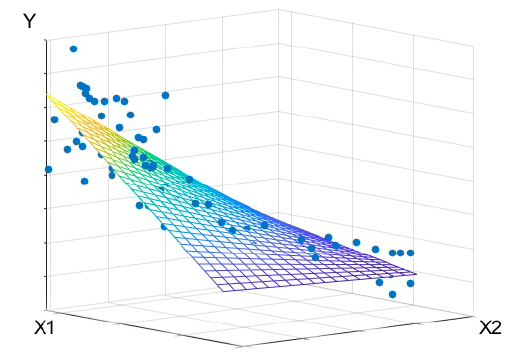
\includegraphics[width=\textwidth]{figures/hyperplane_linear_regression.PNG}
    \end{minipage}   
\end{center}


\vspace{-5pt}

$\rightarrow$ The dimension of the hyperplane of the regression is its \textbf{complexity}.


\vspace{3pt}

\textbf{\underline{Variations:}} 
There are extensions of Linear Regression training called \textbf{regularization}
methods, that aim to \textbf{reduce the complexity} of the models or to address over-fitting in ML. \textit{The regularizer is not dependent on the data.}
$\rightarrow$ In relation to the bias-variance trade-off, regularization aims to decrease complexity in a way that \textbf{significantly reduces variances} while only \textbf{slightly increasing bias}. 


$\rightarrow$ Standardize numeric variables when using regularization because to ensure that 0 is a neutral value, so a low coefficient means "little effect when deviating from average". So values, and therefore coefficients, are on the same scale (\# of standard deviations), to properly distribute weight between them.

$\rightarrow$ \textbf{Multicollinearity} $\rightarrow$ correlated predictors. \textbf{Problem}: Which coefficient gets the common effect? To \textbf{solve}: Loss and Regularization comes. \\


\begin{itemize}

     \item \textbf{Ridge Regression} (L2 regularization): where OLS is modified to minimize the \textbf{squared} sum of the coefficients 
     \vspace{-4pt}
    \[ \boxed{\sum^{n}_{i=1} (y_{i} - \beta_{0} - \sum^{p}_{j=1} \beta_{j} x_{ij})^{2} + \lambda \sum^{p}_{j=1} \beta^{2}_{j} = RSS + \lambda \sum^{p}_{j=1} \beta^{2}_{j}} \]
    \vspace{-7pt}
    
   $\rightarrow$ Prevents the weights from getting too large (L2 norm). If lambda is \textbf{very large then it will add too much weight} and it will lead to \textbf{under-fit}.
   \vspace{-5pt}
   \[ \boxed{ \lambda \propto \frac{1} {\text{model variance}}}  \]
    
    \item \textbf{Lasso Regression} (L1 regularization) : where OLS is modified to minimize the sum of the coefficients 
    \vspace{-3pt}
    \[ \boxed{\sum^{n}_{i=1} (y_{i} - \beta_{0} - \sum^{p}_{j=1} \beta_{j} x_{ij})^{2} + \lambda \sum^{p}_{j=1} \left| \beta_{j} \right| = RSS + \lambda \sum^{p}_{j=1} \left| \beta_{j} \right|}  \]
    \vspace{-10pt}
     
    where $p$ is the no. features (or dimensions), $\lambda \geq 0$ is a tuning parameters to be determined. 
    
    \vspace{2pt}
    
   $\rightarrow$ Lasso shrinks the less important feature’s coefficient to \textbf{zero} thus, removing some feature altogether. If lambda is \textbf{very large value will make coefficients zero} hence it will \textbf{under-fit}.
   \vspace{-3pt}
\end{itemize}

$\rightarrow$ L1 is less likely to shrink coefficients to 0. Therefore L1 regularization leads to sparser models. \\







\subsubsection{Logistic Regression} {\color{teal}\hrule height 0.5pt} \smallskip



\textcolor{blue}{\textbf{Log-Odds} and \textbf{Logistics}} 

\vspace{2pt}
$\bullet$ \textbf{Odds} \\
The probability of success $P(S)$:  \( 0 \leq p \leq 1\)\\
$\rightarrow$ The odds of success are defined as the ratio of the \textbf{probability of success} over the \textbf{probability of failure}. \\
The \textbf{odds} of success: \( \text{Odds}(S) = \frac{P(S)}{P(S^{c})} = \frac{P(S)}{1-P(S)} \) \\
$\rightarrow$ Ex: Odds(failure) = x $\rightarrow$ means x:1 aganist success \\

\vspace{3pt}
$\bullet$ \textbf{Log Odds} or \textbf{logit} $\rightarrow$
\vspace{-7pt}
\[\text{log Odds}(A) = \text{log} \frac{P(A)}{1-P(A)} = \text{log}P(A) - \text{log}\left(1-P(A) \right) \]
\vspace{-7pt}

\vspace{3pt}
$\bullet$ \textbf{Logistic}: The inverse of the logit (logit$^-1$): 
\vspace{-3pt}
\[\boxed{\text{logistic}(x) = \frac{1}{1+e^{-x}} = \frac{e^{x}}{e^{x} +1} }\]

\vspace{-3pt}


\begin{minipage}{0.5\linewidth}
% \begin{figure}[h!]
    \centering
    % \begin{minipage}[b]{\textwidth}
    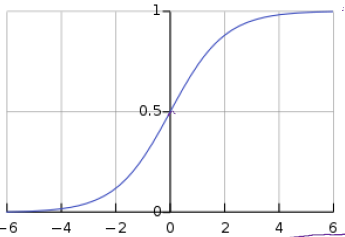
\includegraphics[width=\textwidth]{figures/Logistics_sigmoid_curve.PNG}
    % \caption{ML Production}
    % \label{fig:ML_Production}
    % \end{minipage}
% \end{figure}
\end{minipage}
\textbf{sigmoid} or logistic curve. \\

\vspace{3pt}
$\rightarrow$ Odds are another way of representing probabilities.\\
$\rightarrow$ The logistic and logit functions convert between probabilities and log-odds. \\



\vspace{3pt}
$\bullet$ \textbf{General Linear Models (GLMs)}: 
\vspace{-3pt}
\[\hat{y_{i}} = g^{-1}\left(\beta_{0} + \beta_{1} x_{i1} + \beta_{2} x_{i2} \cdots + \beta_{p} x_{ip} \right) \]
\vspace{-5pt}
\[\boxed{\hat{y}_{i} = g^{-1}\left(\beta_{0} + \sum_{j=1}^{p} \beta_{j} x_{ij}  \right)}\]

Here, $g$ is a link function 
\\

$\bullet$ \textbf{Counts}: Poision regression, log link func \\
$\bullet$ \textbf{Binary}: Logistic regression, logit link  func and $g^{-1}$ is logistic func \\


$\rightarrow$ In logistic regression, a linear output is converted into a probability between 0 and 1 using the sigmoid or logistic function. 
\vspace{-4pt}
\[\boxed{P(y_{i}=1|X) = \hat{y}_{i} = \text{logistic} \left(\beta_{0} + \sum_{j} \beta_{j} x_{ij} \ \right)} \]

\vspace{-3pt}
\[\boxed{ p(X) = \frac{e^{\beta_{0} + \beta_{1}x_{1} + \cdots + \beta_{i} x_{i}}}{1 + e^{\beta_{0} + \beta_{1}x_{1} + \cdots + \beta_{i} x_{i}}}  = p(y = 1 \, | \, X)}\] \




\textbf{\textcolor{blue}{Note :} Coefficients} are linearly related to odds, such that a one unit increase in $x_{1}$ affects odds by $e^{\beta_{1}}$. \\

\textbf{\textcolor{blue}{Note :}} The \textbf{coefficients in logistic regression are interpreted} in terms of their effect on the log-odds of the outcome, and the exponentiated coefficients (odds ratios) provide a clearer understanding of the change in odds associated with each predictor.



\vspace{-5pt}
\begin{center}
    \begin{minipage}{0.86\linewidth}
    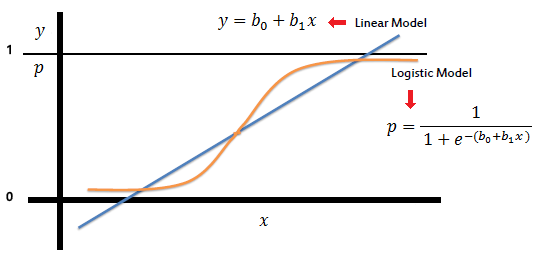
\includegraphics[width=\textwidth]{figures/logistic_function_regression.PNG}
    \end{minipage}
\end{center}

\vspace{-5pt}
The representation below is an equation with binary output, which actually models the probability of default class: 


\vspace{2pt}
\textbf{\underline{Assumptions:}} \\
- Linear relationship between $X$ and log-odds of $Y$ \\
- Observations must be independent to each other \\
- Low multicollinearity \\



\vspace{2pt}
\textbf{\underline{Learning:}} Learning the logistic regression coefficients is done by: \\

$\rightarrow$ \textbf{Minimizing} the \textbf{logistic loss function} 
\vspace{-5pt}
\[\boxed{\underset{\vec{\beta}} {\arg\min} \sum_{i} \text{log}\big(1+\text{exp}(-y_{i} \vec{\beta}x_{i}) \big)} \] 
$\rightarrow$ \textbf{Maximizing} the \textbf{log likelihood} of the training data given the model 
\vspace{-5pt}
\[\boxed{\underset{\vec{\beta}} {\arg\max} \sum_{i} \text{log} \hspace{2pt} P\left(y_{i} | x_{i}, \vec{\beta} \right)} \]











\subsubsection{Linear Discriminant Analysis} {\color{teal}\hrule height 0.5pt} \smallskip

For \textbf{multiclass classification}, LDA is the preferred linear
technique. \\

\textbf{\underline{Representation:}} LDA representation consists of statistical properties calculated for \textbf{each class}: \textbf{means} and the \textbf{covariance} matrix: 

\vspace{-5pt}


\[\boxed{\mu_{k} = \frac{1}{n_{k}} \sum^{n}_{i=1} x_{i}}   \hspace{15pt} \boxed{\sigma^{2} = \frac{1}{n-k} \sum^{n}_{i=1} (x_{i} - \mu_{k})^{2}} \]

\begin{center}
    \begin{minipage}{0.6\linewidth}
        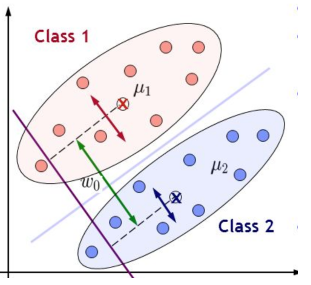
\includegraphics[width=\textwidth]{figures/linear_discriminant_analysis.PNG}
    \end{minipage}
\end{center}


LDA assumes \textbf{Gaussian} data and attributes of \textbf{same} $\sigma^{2}$. 
\vspace{3pt}
\textbf{Predictions} are made using \textbf{Bayes Theorem}: 
\vspace{-4pt}
\[\boxed{ P(y=k \, | \,  X=x) = \frac{P(k) \times P(x|k)}{\sum^{k}_{l=1} P(l) \times P(x|l) } } \]

to obtain a discriminate function (latent variable) for each class $k$, estimating $P(x|k)$ with a \textbf{Gaussian} distribution:
\vspace{-4pt}
\[\boxed{ D_{k}(x) = x \times \frac{\mu_{k}}{\sigma^{2}} - \frac{\mu_{k}^{2}}{2 \sigma^{2}} + ln(P(k))} \]
The class with largest \textbf{discriminant value} is the \textbf{output class}. 


\vspace{3pt}

\textbf{\underline{Variations:}}
\begin{enumerate}
    \item \textbf{Quadratic DA:} Each class uses its own variance estimate
    \vspace{-2pt}
    \item \textbf{Regularized DA:}  Regularization into the variance estimate.
\end{enumerate}


\subsubsection{Data preparation for Linear Algorithm} {\color{teal}\hrule height 0.5pt} \smallskip

\begin{enumerate}
    \item \textbf{Data Transformation:} 
    Linear algorithms require data to have a linear relationship between features and the target variable. Often, transformations like log or polynomial are applied to make the data fit a linear pattern.
    
    \item \textbf{Feature Engineering:} 
    Feature engineering is crucial. Polynomial features or interaction terms may need to be added manually to capture relationships in the data.

    \item \textbf{Handling Outliers:} 
    Linear models are sensitive to outliers. Detecting and either removing or transforming outliers is important, as they can significantly influence the results.

    \item \textbf{Rescaling:} 
    Rescaling features (standardization or normalization) is required to ensure that all features contribute equally to the model. Algorithms such as linear regression perform better with rescaled data.

    \item \textbf{Assumptions:} 
    Linear algorithms assume a linear relationship between the input features and the output variable. Violating this assumption can lead to suboptimal performance.
\end{enumerate}


\subsubsection{Advantages of Linear Algorithms} {\color{teal}\hrule height 0.5pt} \smallskip


\begin{enumerate}
    \item \textbf{Simplicity and Interpretability:} 
    Easy to understand and interpret results (e.g., coefficients indicate feature importance).
    
    \item \textbf{Computational Efficiency:} 
    Faster to train and predict, especially with large datasets.
    
    \item \textbf{Less Prone to Overfitting:} 
    With proper regularization (like Lasso or Ridge), linear models can generalize well on unseen data.
    
    \item \textbf{Strong Theoretical Foundation:} 
    Well-established statistical properties and a solid theoretical framework.
    
    \item \textbf{Works Well with Linearly Separable Data:} 
    Performs well when the relationship between features and target variable is linear.
\end{enumerate}
\vspace{5pt}

\vspace*{\fill}

\columnbreak

\subsection{Nonlinear Algorithms} {\color{teal}\hrule height 1pt} \smallskip
All Nonlinear Algorithms are non-parametric and more flexible. They are not sensible to outliers and do not require any shape of distribution. 

\subsubsection{Naive Bayes Classifier} {\color{teal}\hrule height 0.5pt} \smallskip

Naive Bayes is a \textbf{classification} algorithm interested in
selecting the \textbf{best hypothesis} $h$ given data $X$ \textbf{assuming that the features of each data point are all independent}  \\

\textbf{\underline{Representation:}} 
The representation is based on Bayes Theorem:
\vspace{-3pt}
\[\boxed{P(Y|X) = \frac{P(X|Y) \times P(Y)}{P(X)}} \]
With naive hypothesis, \(P(Y|X) = P(x_{1}, x_{2}, \cdots, x_{i} | \, Y) = P(x_{1} | Y) \times P(x_{1} | Y) \times \cdots P(x_{i} | Y) \) 
\vspace{-3pt}
\[\boxed{P(X|Y) = \prod^{n}_{i=1} P(x_{i} | \, Y)} \]

\vspace{3pt}
The prediction is the maximum a \textbf{posterior hypothesis}:
\vspace{-3pt}
\[\boxed{\text{max}\left(P(Y|X)\right) = \text{max}\left(P(X|Y) \times P(Y)\right)} \] 
here, the denominator is not kept as it is only for normalization.

\vspace{3pt}
\textbf{\underline{Learning:}} Training is \textbf{fast} because only \textbf{probabilities} need to be calculated: 
\vspace{-3pt}
\[\boxed{P(Y) = \frac{\text{instances}_{Y}}{ \text{all instances}}} \hspace{15pt} \boxed{P(x|Y) = \frac{\text{count}(x \land Y  )}{\text{instances}_{Y}}}\]



\vspace{3pt} 
\textbf{\underline{Variations:}} \textbf{Gaussian Naive Bayes} can extend to numerical attributes by assuming a Gaussian distribution. Instead of $P(x|h)$ are calculated with $P(h)$ during \textbf{learning}, and MAP for \textbf{prediction} is calculated using Gaussian PDF
\vspace{-3pt}
\[\boxed{f(x \, | \,  \mu(x), \sigma) = \frac{1}{\sqrt{2 \pi \sigma^{2}}} e^-{\frac{(x-\mu)^{2}}{2\sigma^{2}}} }\]
\vspace{-3pt}
\[\mu(x) = \frac{1}{n} \sum^{n}_{i=1} x_{i} \hspace{10pt}  \sigma = \sqrt{\frac{1}{n} \sum^{n}_{i=1} \left( x_{i} - \mu(x) \right)^{2}} \]







% \vspace{3pt}
% \subsubsection{Likelihood and Posterior} 
% \[\boxed{\mathcolor{orange}{P(\theta |\textbf{y})} = \frac{\mathcolor{green}{P(\textbf{y}|\theta)} \, \mathcolor{purple}{P(\theta)} }{P(\textbf{y})}} \]
% \vspace{-10pt}

% • \mathcolor{purple}{$P(\theta)$} is the \textcolor{purple}{prior}
% \\

% • \mathcolor{green}{$P(y | \theta)$} is the \textcolor{green}{likelihood} – how likely is the data given params $\theta$ \\
% • $P(y) = \int P(y | \theta) P(\theta) d\theta $ is a scaling factor (constant for fixed $y$) \\
% • $\mathcolor{orange}{P(\theta | y)}$ is the \textcolor{orange}{posterior}.


% \vspace{3pt}
% • We’re maximizing likelihood (ML estimator) \\
% • Can also maximize posterior (MAP estimator)\\
% \hspace{7pt} • When prior is constant, they’re the same\\
% \hspace{7pt} • With lots of data, they’re almost the same\\




% \begin{center}
%     \begin{minipage}{0.8\linewidth}
%         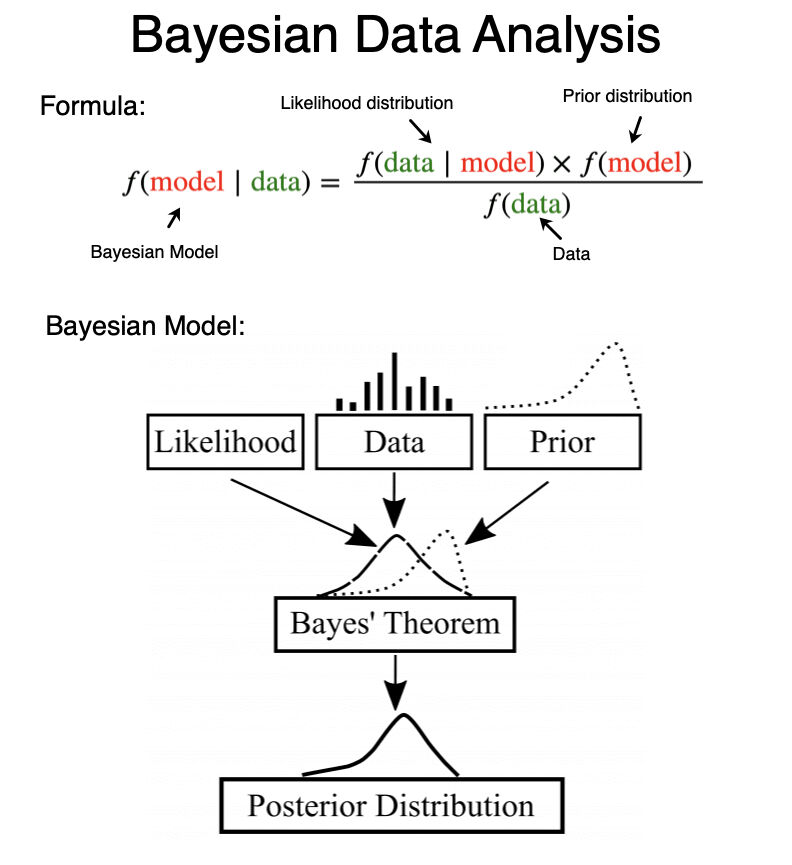
\includegraphics[width=\textwidth]{figures/Bayesian_data_analysis.jpeg}
%     \end{minipage}
% \end{center}


% \begin{center}
%     \begin{minipage}{\linewidth}
%         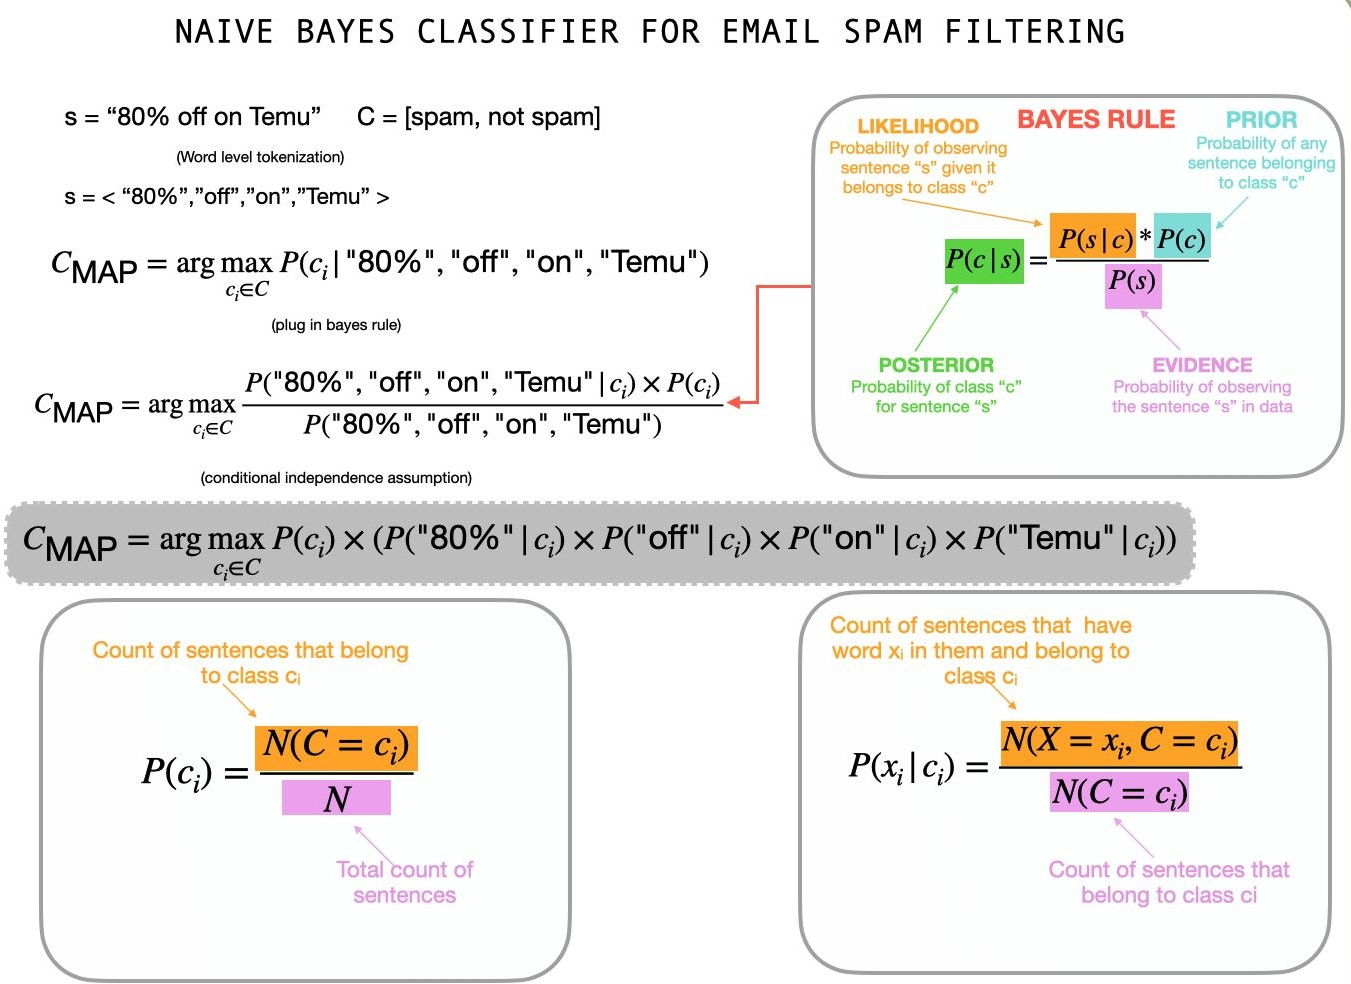
\includegraphics[width=\textwidth]{figures/Naive Bayes Spam Classifier.jpg}
%     \end{minipage}
% \end{center}


% \vspace*{\fill}
% \columnbreak


\subsubsection{Support Vector Machines} {\color{teal}\hrule height 0.5pt} \smallskip

SVM is a go-to for high performance with little tuning. Compares extreme values in your dataset. \\

\vspace{3pt}

In SVM, a \textbf{hyperplane} (or decision boundary: $w^{T}x - b = 0$) is selected to \textbf{separate the points} in the input variables space by their class, with the \textbf{largest margin}. The closest datapoints (defining the margin) are called the
\textbf{support vectors}. \\

% But real data cannot be perfectly separated, that is why a
% $C$ defines the amount of violation of the margin allowed. The lower $C$, the more sensitive SVM is to training data. \\

\vspace{3pt}
$\rightarrow$ The \textbf{goal} of a support vector machine is to find the optimal separating hyperplane which maximizes the \textbf{margin} of the training data.

\vspace{-10pt}
\begin{center}
    \begin{minipage}{0.65\linewidth}
    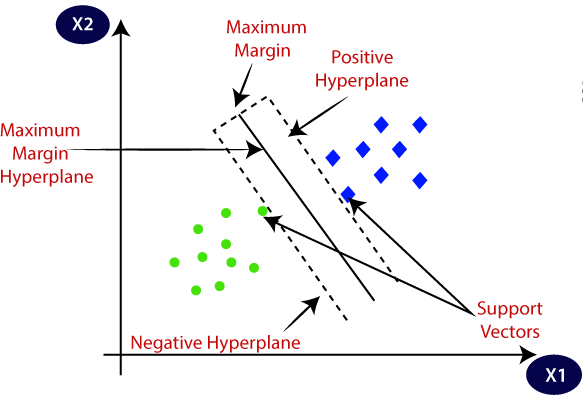
\includegraphics[width=\textwidth]{figures/svm_figure.PNG}
    \end{minipage}
\end{center}

\vspace{-10pt}

\begin{center}
    \begin{minipage}{0.8\linewidth}
    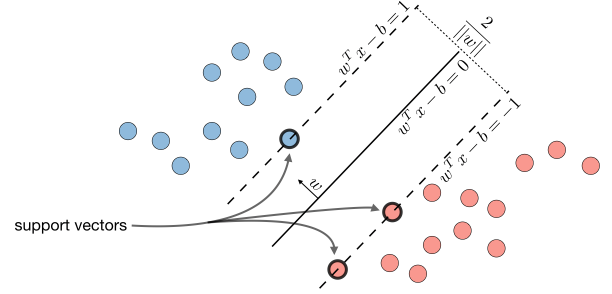
\includegraphics[width=\textwidth]{figures/svm_figures2.PNG}
    \end{minipage}
\end{center}
\vspace{-5pt}

The \textbf{prediction} function is the signed \textbf{distance} of the new input $x$ to the separating hyperplane $w$, \textcolor{blue}{with b the bias}: 
\vspace{-4pt}
\[\boxed{f(x) = \langle w,x\rangle + b = w^{T} x + b} \] 
\vspace{-5pt}




% which gives for \textbf{linear kernel}, with $x_{i}$ the support vectors:
% \[ f(x) = \sum^{n}_{i=1} a_{i} \times () \]

\vspace{3pt}
$\rightarrow$ \textbf{Optimal margin classifier: } The optimal margin classifier $h$ is such that: 
\vspace{-4pt}
\[\boxed{h(x) = \text{sign}(w^{T}x - b)} \]
where $(w, b) \in \mathcal{R}^{n} \times \mathcal{R}$ is the  solution of the following optimization problem:
\vspace{-4pt}
\[ \boxed{\text{min}\frac{1}{2} \lVert {w} \rVert^{2} }\] such that \hspace{5pt} \[\boxed{y^{(i)} (w^{T}x^{(i)} - b) \geq 1}\]

\vspace{3pt}


\textbf{\underline{Learning:}} \\
$\rightarrow$ \textbf{Hinge loss : } The hinge loss is used in the setting of SVMs and is defined as follows:
\vspace{-2pt}
\[\boxed{L(\hat{y},y) = \left[1 - y\hat{y}  \right]_{+} = \text{max}(0, \, 1-y\hat{y})} \]

\vspace{3pt}
$\rightarrow$ \textbf{Lagrangian : } We define the Lagrangian $\mathcal{L}(w, b)$ as follows:
\vspace{-3pt}
\[\boxed{\mathcal{L}(w, b) = f(w) + \sum^{l}_{i=1} \beta_{i} h_{i} (w) }\]


Lagrange method is required to convert constrained optimization problem into unconstrained optimization problem. The goal of above equation to get the optimal value for \textbf{w} and \textbf{b}.
\vspace{-4pt}
\[\boxed{ \lambda \lVert \vec{w} \rVert^{2} + \left[ \frac{1}{n} \sum^{n}_{i=1} \text{max} \big(0, \, 1 - y_{i}(\vec{w} \cdot \vec{x_{i}} - b) \big)\right] }  \] 
The\textbf{ first term} is the regularization term, which is a technique to avoid overfitting by penalizing large coefficients in the solution vector. The \textbf{second term}, hinge loss, is to penalize misclassifications. It measures the error due to misclassification (or data points being closer to the classification boundary than the margin).  The $\lambda$ is the regularization coefficient, and its major role is to determine the trade-off between increasing the margin size and ensuring that the $x_{i}$ lies on the correct side of the margin.




\vspace{3pt}
$\rightarrow$ \textbf{Kernel : } A kernel is a way of computing the dot product of two vectors $\textbf{x}x$ and $\textbf{y}y$ in some (possibly very high dimensional) feature space, which is why kernel functions are sometime called "generalized dot product". The kernel trick is a method of using a linear classifier to solve a non-linear problem by transforming linearly inseparable data to linearly separable ones in a higher dimension.\\

\vspace{3pt}
Given a feature mapping $\phi$, we define the kernel $K$ as follows:
\vspace{-4pt}
\[\boxed{K(x, z) = \phi(x)^{T} \phi(z)} \] 
In practice, the kernel $K$ defined by $\boxed{K(x, z) =  e^-{\frac{\lVert x - z \rVert^{2}}{2\sigma^{2}}}}$ is called the Gaussian kernel and is commonly used.

\vspace{-5pt}
\begin{center}
    \begin{minipage}{0.9\linewidth}
    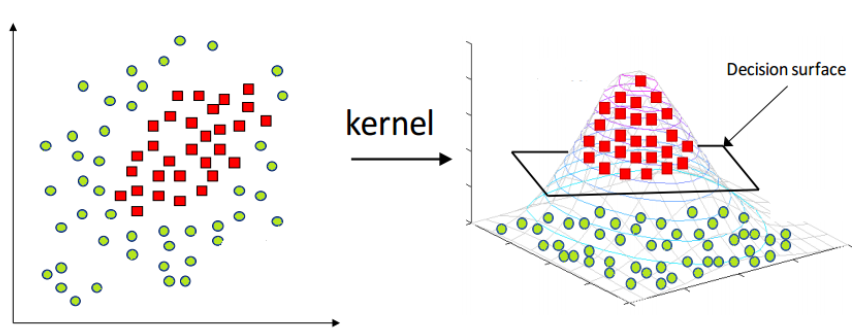
\includegraphics[width=\textwidth]{figures/kernel_SVM.PNG}
    \end{minipage}
\end{center}

\vspace{-5pt}

\textbf{\textcolor{blue}{Note: }} we say that we use the "kernel trick" to compute the cost function using the kernel because we actually don't need to know the explicit mapping $\phi$, which is often very complicated. Instead, only the values $K(x,z)$ are needed.



\vspace{3pt}
\textbf{\underline{Variations:}} \\
SVM is implemented using various kernels, which define the
measure between new data and support vectors:
\vspace{-3pt}
\begin{enumerate}
    \item \textbf{Linear} (dot-product):  \hspace{5pt} \(\boxed{K(x, x_{i}) = \sum(x \times x_{i})} \)
    \vspace{-3pt}
    \item \textbf{Polynomial:}  \hspace{38pt} \( \boxed{K(x, x_{i}) = 1 + \sum(x \times x_{i})^{d} }\)
    \vspace{-3pt}
    \item \textbf{Radial:}  \hspace{55pt} \(\boxed{K(x, x_{i}) = e^-{\gamma \sum (x - x_{i})^{2}}}\)
\end{enumerate}




\textbf{\textcolor{blue}{Hyperparameters}}: regularization parameter (C) and the kernel parameters (such as gamma for the RBF kernel).



% \vspace*{\fill}

% \columnbreak




\subsubsection{K-Nearest Neighbors} {\color{teal}\hrule height 0.5pt} \smallskip

\textbf{If you are similar to your neighbors, you are one of them.}
KNN uses the \textbf{entire training data}, \textbf{no training} is required. 


\textbf{\textcolor{blue}{Note: }} Higher $k$ $\rightarrow$ higher the bias, Lower $k$ $\rightarrow$ higher the variance.

$\bullet$ \textbf{Choice of \textbf{k} is very critical} $\rightarrow$ A small value of \textbf{k} means that noise will have a higher influence on the result. 
$\rightarrow$ A large value of \textbf{k} make everything classified as the most probable class and also computationally expensive.\\

$\rightarrow$ A simple approach to \textbf{select} \textbf{k} is set $\boxed{\text{k} = \sqrt{n}}$ or \textbf{cross-validating} on small subset of training data (validation data) by \textbf{varying} values of $k$ and \textbf{observing} training - validation error. \\

$\rightarrow$ \textcolor{purple}{Minkowski Distance} = \(\boxed{\left(\sum| a_{i} - b_{i}|^{p}\right)^{\frac{1}{p}}} \) \\
\hspace{10pt} - p=1 gives \textbf{Manhattan distance} \(\boxed{\sum|a_{i} - b_{i}|} \)  \\
\hspace{10pt} - p=2 gives Euclidean distance \(\boxed{\sqrt{\sum(a_{i} - b_{i})^{2}}} \)\\

\vspace{2pt}
$\rightarrow$ \textcolor{purple}{Hamming Distance} - count of the differences between two vectors, often used to compare categorical variables.



\begin{center}
    \begin{minipage}{\linewidth}
    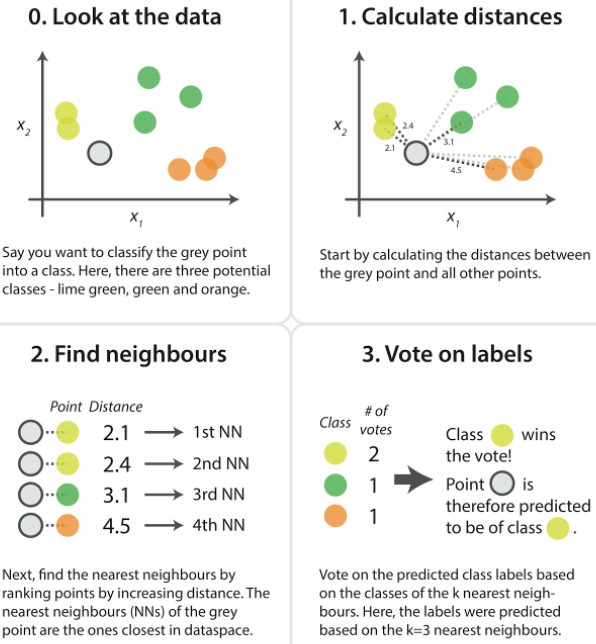
\includegraphics[width=\textwidth]{figures/knn_steps.PNG}
    \end{minipage}
\end{center}











 
% \textbf{Time complexity:}
% The distance calculation step requires quadratic time complexity, and the sorting of the calculated distances requires an \(O(N \text{log} N)\) time. Total process is an \(O(N^{3} \text{log} N)\)  \\
% \vspace{2pt}
% \textbf{Space complexity:}
% Since it stores all the pairwise distances and is sorted in memory on a machine, memory is also the problem. Usually, local machines will crash, if we have very large datasets.

 
 




\subsubsection{Classification and Regression Trees (CART)} {\color{teal}\hrule height 0.5pt} \smallskip

Decision Tree is a \textbf{Supervised learning} technique that can be used for both \textbf{Classification} and \textbf{Regression} problems. 



\vspace{-5pt}
\begin{center}
    \begin{minipage}{0.75\linewidth}
    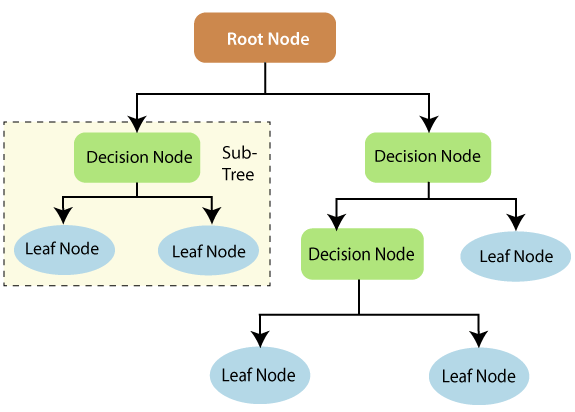
\includegraphics[width=\textwidth]{figures/decision_trees.PNG}
    \end{minipage}
\end{center}
\vspace{-7pt}


Here, each \textbf{node} represents a question about the data, and the \textbf{branches} from each node represent the possible answers.


$\rightarrow$ \textbf{Root Node}: It is the very first node (parent node), and denotes the whole population, and gets split into two or more Decision nodes based on the feature values. \\
$\rightarrow$ \textbf{Decision Node}: At each decision node, the algorithm chooses the best feature and threshold to split the data, aiming to create the most homogeneous subsets. They have \textbf{multiple} branches.  \\

$\rightarrow$ This process continues until a stopping condition is met (like maximum depth or pure leaves). \\

$\rightarrow$ \textbf{Leaf Node}: The final predictions are made at the leaf nodes, which represent the outcome of those \textbf{decisions}.

$\rightarrow$ \textbf{Sub-Tree}: A branch is a subdivision of a complete tree. 


\vspace{3pt}
At each leaf node, CART predicts the most frequent category, assuming false negative and false positive costs are the same. \\

$\rightarrow$ The splitting process handles multicollinearity and outliers. \\
$\rightarrow$ Trees are prone to high variance, so tune through CV.

\vspace{2pt}
\textcolor{blue}{Note:} In decision trees, the \textbf{depth of the tree} determines the variance. Decision trees are commonly pruned to control variance


\vspace{3pt} 


$\bullet$ CART for \textcolor{blue}{regression } \textbf{minimizes SSE} by splitting data into sub-regions and predicting the average value at leaf nodes. The complexity parameter $cp$ only keeps splits that reduce loss by at least $cp$ (small $cp$ $\rightarrow$ deep tree). 

\vspace{2pt}
$\bullet$ CART for \textcolor{blue}{classification }
\textbf{minimizes the sum of region impurity}, where $p_{i}$ is the probability of a sample being in category $i$. Possible measures, each with a max impurity of 0.5.
\\

- \( \boxed{\text{Gini Impurity / Gini Index / Gini Coefficient} = 1 - \sum(p_{i})^{2}} \) \\
- \(\boxed{
\text{Cross Entropy} = \sum(p_{i})\text{log}_{2}(p_{i})} \)



\vspace{3pt}
\textbf{\textcolor{blue}{Procedure}}:
\vspace{-3pt}
\begin{enumerate}
    \item Calculate entropy of the \textbf{outcome} classes (c) \(\boxed{E(T) = \sum^{c}_{i=1} -p_{i} \, \text{log}_{2}p_{i}} \)
    \vspace{-2pt}
    \item The dataset is split on the different attributes. The entropy of each branch is calculated. Then it is added proportionally to get \textbf{total entropy for the split}. The resulting entropy is subtracted from the entropy before the split.
    \vspace{-3pt}
    \[\boxed{\text{Gain}(T,X) = \text{Entropy}(T) - \text{Entropy}(T, X) }\]
    \vspace{-10pt}
    \item Choose attributes with \textbf{largest information Gain} as the \textbf{decision node}, divide the dataset by its branches and repeat the same process on \textbf{every branch}.
    \vspace{-2pt}
    \item A branch with \textbf{entropy of 0} is a leaf node
    \vspace{-2pt}
    \item A branch with \textbf{entropy more than 0} needs futher splitting.
    \vspace{-2pt}
    \item ID3 algorithm is run recursively on the \textbf{non-leaf branches}, until all data is classified
    \vspace{-2pt}
\end{enumerate}


\textbf{\textcolor{blue}{Hyperparameters}}:  The most common \textbf{Stopping Criterion} for splitting is a minimum of \textbf{training observations per node},  maximum depth of the tree 



\subsubsection{Ensemble Algorithms} {\color{teal}\hrule height 0.5pt} \smallskip

Ensemble methods combine multiple, simpler algorithms (weak learners) to obtain better performance algorithm.
\vspace{-5pt}
\begin{center}
        \footnotesize
        \begin{tabular}{ c|c }
           \textbf{Bagging} & \textbf{Boosting} \\
           \hline
          & AdaBoost \\
          Random Forest & Gradient Boosting \\
          & XGBoost \\
        \end{tabular}
\end{center}
\vspace{-5pt}

$\bullet$ \textbf{\textcolor{purple}{Bagging}} \\
$\rightarrow$ It involves \textbf{parallel} training of multiple models independently on \textbf{different subsets} of the data. These subsets of data are drawn using the bootstrap technique. \\
$\rightarrow$ Then averaging their predictions (for regression) or majority voting (for classification). \\
$\rightarrow$ It can \textbf{reduce the variance} and prevent overfitting by averaging out the errors of individual models.

\vspace{3pt}
$\rightarrow$ \textbf{\textcolor{blue}{Bootstrapping}} is drawing random \textbf{sub-samples} (sampling \textbf{with replacement}) from a large \textbf{sample} (available data) to estimate quantity (parameters) of a unknown population by \textbf{averaging the estimates} from these \textbf{sub-samples}. \\









\vspace{3pt}
\textcolor{teal}{\textbf{Random Forest}} \\
$\rightarrow$\textbf{ Bagged Decision Trees}: Each DT may contain different no. of rows and different no. of features. \\
$\rightarrow$ Individual DTs may face \textbf{overfitting} i.e. have \textbf{low bias} (complex model) but \textbf{high variance}, by ensembling a lot of DTs we are going to \textbf{reduce the variance}, while not increasing the bias. \\ 
\textbf{\textcolor{blue}{Hyperparameters}}: number of trees, maximum depth of the trees 

\vspace{7pt}
$\bullet$ \textbf{\textcolor{purple}{Boosting}} \\
$\rightarrow$ It involves \textbf{sequentially} training of multiple models, where each model tries to correct the errors of the previous ones.



\vspace{-5pt}
\begin{center}
    \begin{minipage}{\linewidth}
    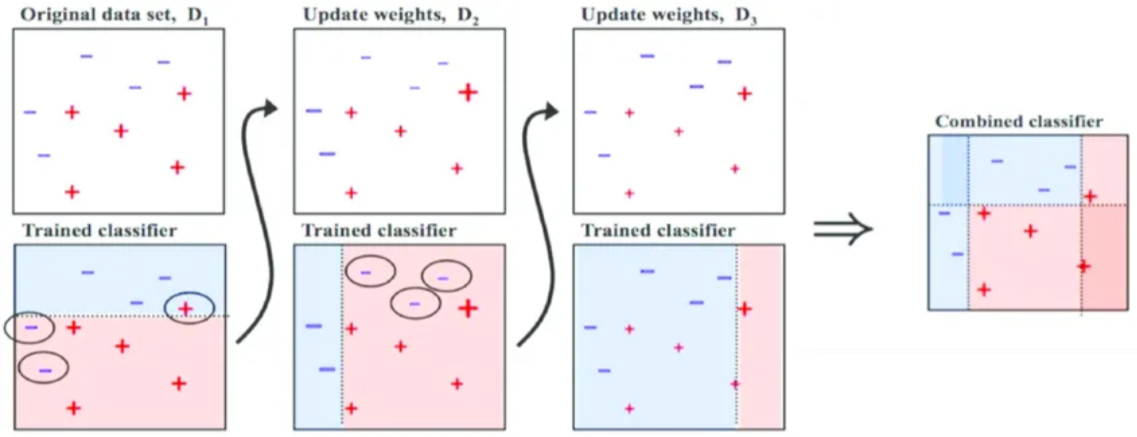
\includegraphics[width=\textwidth]{figures/boosting.PNG}
    \end{minipage}
\end{center}
\vspace{-5pt}



\vspace{3pt}
\textcolor{teal}{\textbf{AdaBoost}} \\

$\bullet$ Uses the \textbf{same training samples} at each stage \\
$\bullet$ "Weakness" =  Misclassified data points \\
$\bullet$ \textbf{Learning Focus}: Primarily reduces bias (increases variance) by focusing on misclassified instances
\textbf{Algorithm}:
\vspace{-3pt}
\begin{enumerate}
    \item \textbf{Initialize Weights}: Assign \textbf{equal weight} to each of the training data 
    \vspace{-3pt}
    \item \textbf{Train weak model and Evaluate}: Provide this as input to the weak model and identify the wrongly classified data points
    \vspace{-3pt}
    \item \textbf{Adjust Weights}: Increase the weight of wrongly classified data points
      \vspace{-3pt}
    \item \textbf{Combined Models}: Combine the weak models using a weighted sum, where weights are based on the accuracy of each learner.
    \vspace{-3pt}
    \item Repeat steps 2-4 for a predefined number of iterations or until the error is minimized.
\end{enumerate}
$\bullet$ \textbf{Limitations}: Sensitive to noisy data and outliers since misclassified points are given more focus. \\

\textbf{\textcolor{blue}{Hyperparameters}}: number of estimators, learning rate.


\vspace{3pt}
\textcolor{teal}{\textbf{Gradient Boosting}} \\
$\bullet$ Uses the \textbf{different training samples} at each stage \\
$\bullet$ "Weakness" =  Residuals or Erros \\
$\bullet$ \textbf{Learning Focus}: Instead of adjusting weights, it optimizes the model by minimizing a loss function (e.g., mean squared error for regression).\\
\textbf{Algorithm}:
\vspace{-3pt}
\begin{enumerate}
    \item \textbf{Initialize Model}: Start with an initial model (e.g., a constant value). \textcolor{blue}{Let's say Avg.}
    \vspace{-3pt}
    \item \textbf{Compute Residuals}: Calculate the residuals (errors) of the current model.
    \vspace{-3pt}
    \item \textbf{Train Weak Learner}: Train a weak learner on the residuals.
    \vspace{-3pt}
    \item \textbf{Update Model}: Add the weak learner to the model with a certain learning rate.
    \vspace{-3pt}
    \item Repeat steps 2-4 for a fixed number of iterations or until the model converges.
\end{enumerate}
$\bullet$ \textbf{Limitations}: Slower to train and more prone to overfitting without careful tuning.

\textbf{\textcolor{blue}{Hyperparameters}}: learning rate, number of boosting stages, maximum depth of individual trees.




\vspace{3pt}
\textcolor{teal}{\textbf{XGBoost}} \\
$\bullet$ Enhances gradient boosting by making it faster, more efficient, and more accurate.. \\
$\rightarrow$ \textbf{Execution speed}: Parallelization (It will use all cores of CPU), Cache optimization, Out of memory (Data size bigger than memory) \\

$\rightarrow$ \textbf{Model performance: }  \\
\hspace{8pt}- Adds regularization to balance the trade-off between fitting the training data and maintaining model simplicity. \\
\hspace{8pt}- \textbf{Auto pruning}: Prevents trees from growing too large, improving generalization and reducing the risk of overfitting. \\
\hspace{8pt}- During training, model learns the optimal way to split data with \textbf{missing values} as well as model learns from the patterns of \textbf{missing data} and adjusts the decision boundaries accordingly.\\
\hspace{8pt}- Efficient handling of sparse data \\
\hspace{8pt}- Flexible: Supports a variety of loss functions and custom objective functions \\

\textbf{\textcolor{blue}{Hyperparameters}}: Learning Rate, Number of Trees, Maximum Depth, Min Child Weight, Subsample, Booster Type, Early Stopping Rounds


\subsubsection{Data Preparation for Non-Linear Algorithms} {\color{teal}\hrule height 0.5pt} \smallskip

\begin{enumerate}
    \item \textbf{Data Transformation:} 
    Non-linear algorithms can naturally model non-linear relationships without the need for data transformations, as they are capable of capturing complex patterns.

    \item \textbf{Feature Engineering:} 
    Non-linear models are less reliant on manual feature engineering. Algorithms like decision trees or neural networks can automatically capture feature interactions and non-linear relationships.

    \item \textbf{Handling Outliers:} 
    Non-linear algorithms, such as decision trees and support vector machines, are generally more robust to outliers compared to linear models.

    \item \textbf{Rescaling:} 
    Some non-linear models (e.g., neural networks, support vector machines) benefit from rescaling, while others (e.g., decision trees, random forests) do not require rescaling.

    \item \textbf{Assumptions:} 
    Non-linear algorithms do not assume a linear relationship between inputs and outputs, allowing them to model more complex relationships in the data without predefined structures.
\end{enumerate}



\subsubsection{Advantages of Non-Linear Algorithms} {\color{teal}\hrule height 0.5pt} \smallskip
\begin{enumerate}
    \item \textbf{Captures Complex Relationships:} 
    Can model intricate patterns and interactions in the data that linear algorithms might miss.
    
    \item \textbf{Higher Flexibility:} 
    Adaptable to various data types and structures (e.g., images, text).
    
    \item \textbf{Improved Accuracy:} 
    Often yields better performance on non-linear datasets by fitting the data more closely.
    
    \item \textbf{Handles High Dimensionality:} 
    Suitable for high-dimensional spaces, especially with techniques like kernel methods or neural networks.
    
    \item \textbf{No Assumption of Linearity:} 
    Does not require prior knowledge of the relationship between input features and output, making it versatile.
    
    \item \textbf{Feature Engineering Not Always Necessary:} 
    Some non-linear algorithms, like tree-based models, automatically capture interactions and non-linearities without explicit feature engineering.
\end{enumerate}




% \vspace*{\fill}

% \columnbreak


\section{Unsupervised Machine Learning} {\color{teal}\hrule height 1pt} \smallskip
\begin{enumerate}
    \item Clustering
    \vspace{-3pt}
    \item Dimension Reduction
    \vspace{-3pt}
    \item Association Rule Mining
    \vspace{-3pt}
    \item Graphical Modelling and Network Analysis
    \vspace{-3pt}
\end{enumerate}

\subsection{Clustering} {\color{teal}\hrule height 0.5pt} \smallskip

Grouping objects into meaningful \textbf{subets} or, \textbf{clusters}. $\rightarrow$ Objects within each cluster are similar. \\
\textbf{Clustering Algorithms:}
\begin{enumerate}
    \item Partition-based methods
    \vspace{-3pt}
    \begin{enumerate}
    \vspace{-3pt}
        \item K-means clustering
        \vspace{-3pt}
        \item Fuzzy C-Means
        \vspace{-3pt}
    \end{enumerate}
    
    \item Hierarchical methods
    \vspace{-3pt}
    \begin{enumerate}
    \vspace{-3pt}
        \item Agglomerative Clustering
        \vspace{-3pt}
        \item Divisive Clustering
        \vspace{-3pt}
    \end{enumerate}
    
    \item Density-based methods
    \begin{enumerate}
    \vspace{-3pt}
        \item Density-Based methods (DBSCAN)
    \end{enumerate}
\end{enumerate}


\vspace{5pt}

\subsubsection{K-means clustering}  {\color{teal}\hrule height 0.5pt} \smallskip

The objective of K-means clustering is to \textbf{minimize} total \textbf{intra-cluster} or, the \textbf{squared error function.} 
\vspace{-5pt}
\[\text{Objective  function} \rightarrow  \boxed{J = \sum^{K}_{j=1} \sum^{n}_{i=1} \lVert X^{(j)}_{i} -  C_{j} \rVert^{2} }\]

\vspace{-3pt}


Here, $K$ is No. of clusters, $n$ is No. of cases, $C_{j}$ is centroid for cluster $j$

\vspace{-10pt}
\begin{center}
    \begin{minipage}{0.6\linewidth}
    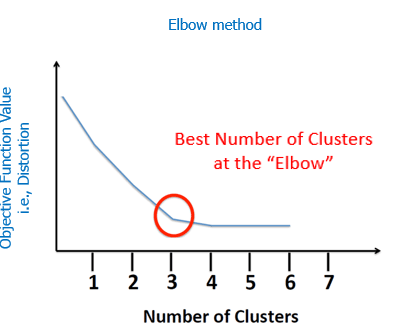
\includegraphics[width=\textwidth]{figures/K_means_clustering.PNG}
    \end{minipage}
\end{center}
\vspace{-5pt}




\begin{enumerate}
    \item Divide data into $K$ clusters or groups.
    \vspace{-3pt}
    \item Randomly select \textbf{centroid} for each of these $K$ clusters.
    \vspace{-3pt}
    \item Assign data points to their closest cluster
    \textbf{centroid} according to Euclidean/ Square Euclidean/Manhattan/Cosine
    \vspace{-3pt}
    \item Calculate the \textbf{centroids} of the newly formed clusters.
    \vspace{-3pt}
    \item Repeat steps 3 and 4 until the \textbf{same centroids} (convergences) are assigned to each cluster.
    \vspace{-3pt}
\end{enumerate}


\begin{center}
    \begin{minipage}{\linewidth}
    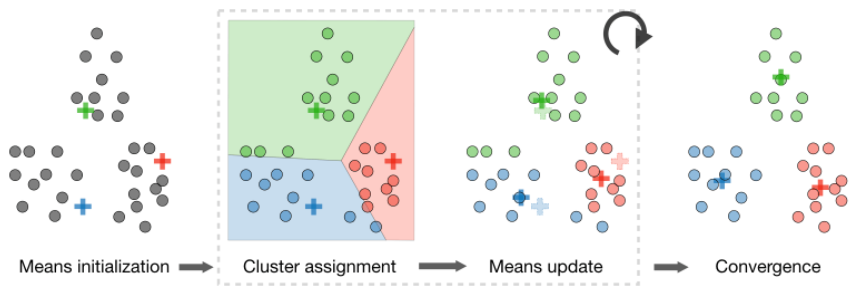
\includegraphics[width=\textwidth]{figures/k_means_cluster_update.PNG}
    \end{minipage}
\end{center}

$\rightarrow$ K-means \textbf{always converges} (mostly to local minimum not to global minimum) \\

$\bullet$ \textbf{How to choose $K$ number of clusters in K-Means algorithm?} \\
$\rightarrow$ The maximum possible number of clusters will be equal to the number of observations in the dataset.



\subsection{Hierarchial Clustering} {\color{teal}\hrule height 0.5pt} \smallskip

\subsubsection{Agglomerative method: "Bottom-up"}
\begin{enumerate}
    \item Compute the distance or, \textbf{proximity matrix}
    \item \textbf{Initialization:} Each observation is a cluster
    \item \textbf{Iteration:} Merge two clusters which are most similar; until \textbf{all observations} are merged into a single cluster.
\end{enumerate}


\subsubsection{Divisive method: "Top-down"}
\begin{enumerate}
    \item Compute the distance, or \textbf{proximity matrix}
    \item \textbf{Initialization:} All objects stay in one cluster
    \item \textbf{Iteration: } Select a cluster and split it into two sub-cluster until each leaf cluster contains only \textbf{one observation}.
\end{enumerate}

\textbf{\textcolor{blue}{Proximity (distance) matrix}} \\
$\rightarrow$ \textbf{\underline{Single or ward linkage: }} Minimize within cluster distance
\vspace{-3pt}
\[\boxed{ L(C_{1}, C_{2}) = min\left[D \left(X^{C_1}_{i}, X^{C_2}_{j}\right) \right]} \]


$\rightarrow$ \textbf{\underline{Complete linkage:}} Longest distance between two points in each cluster. Minimize maximum distance of between cluster pairs
\vspace{-3pt}
\[\boxed{L(C_{1}, C_{2}) = max\left[D \left(X^{C_1}_{i}, X^{C_2}_{j}\right) \right]}  \]


$\rightarrow$ \textbf{\underline{Average linkage:}} Minimize average distance between cluster pairs
\vspace{-3pt}
\[\boxed{L(C_{1}, C_{2}) = \frac{1}{n_{C_1} n_{C_2}} \sum^{n_{C_1}}_{i=1} \sum^{n_{C_2}}_{j=1}  \left[D \left(X^{C_1}_{i}, X^{C_2}_{j}\right) \right]}  \]

\subsection{DBSCAN} {\color{teal}\hrule height 0.5pt} \smallskip

$\rightarrow$ \underline{Two parameters}: $\varepsilon$ - distance, minimum points 

\vspace{2pt}

$\rightarrow$ \underline{Three classifications of points}:

\begin{itemize}
    \vspace{-3pt}
    \item \textbf{Core:} has atleast minimum points within  $\varepsilon$ - distance including itself
    \vspace{-3pt}
    \item $\varepsilon$ - distance has less than minimum points within $\varepsilon$ - distance but can be reached by clusters.
    \vspace{-3pt}
    \item \textbf{Outlier:} point that cannot be reached by cluster
\end{itemize}
\textbf{Procedure:}
\begin{enumerate}
    \item Pick a random point that has not been assigned to a cluster or, designated as an \textbf{Outlier}. Determine if it is a \textbf{Core Point}. If not, label the point as\textbf{ Outlier}.
    \item Once a \textbf{Core Point} has been found, add all directly reachable to its cluster. Then do \textbf{neighbor jumps} to each reachable point and add them to the cluster. If an \textbf{Outlier} has been added, label it as a \textbf{Border Point}.
    \item Repeat these steps until all points are assigned a cluster or, label as \textbf{Outlier}.
\end{enumerate}





\subsection{Dimensionality Reduction Methods} {\color{teal}\hrule height 0.5pt} \smallskip

Reduce the number of input variables (attributes or features) in dataset.

\subsubsection{Principle Component Analysis (PCA)}  {\color{teal}\hrule height 0.5pt} \smallskip

PCA combines highly correlated variables into a new, smaller set of constructs called \textit{ principal components}, which capture most of the variance present in the data.
\begin{itemize}
\vspace{-2pt}
    \item Dimensionality reduction
    \vspace{-2pt}
    \item Feature extraction
    \vspace{-2pt}
    \item Data visualization
    \vspace{-2pt}
\end{itemize}

\underline{Procedure:}
\begin{enumerate}
    \item\textbf{ Standarize} the data: \(\boxed{Z = \frac{X-mean}{SD} } \)
    \vspace{-2pt}
    \item Calculate \textbf{covariance-matrix} of the standarized data 
    \vspace{-2pt}
    \[\boxed{V = \text{cov}(Z^{T})} \]
    \vspace{-2pt}
    \item Find \textbf{eigen-values} and \textbf{eigen-vectors} from the covariance-matrix 
    \vspace{-2pt}
    \[\boxed{\text{values}, \, \text{vectors} = \text{eig}(V)}\]
    \vspace{-2pt}
    \item Feature vectors;  It is simply the matrix that has columns, the eigen-vectors of the components that we decide to keep.
    \vspace{-2pt}
    \item Project data $\rightarrow$ \(\boxed{Z_{\text{new}} = \text{vectors}^{T} \cdot Z^{T}}\)
    \vspace{-2pt}
\end{enumerate}






\subsection{Association Rule Mining} {\color{teal}\hrule height 0.5pt} \smallskip

"Market Basket Analysis" $\rightarrow$ It uses Machine Learning models to analyze data for patterns or, co-occurence in a database.


\subsection{Graphical Modelling and Network Analysis} {\color{teal}\hrule height 0.5pt} \smallskip

"Bayesian Networks"



\vspace*{\fill}



\columnbreak

%%%%%%%%%%%%%%%%%%%%%%%%%%%%%%% Neural Network %%%%%%%%%%%%%%%%%%%%%%
\section{Neural Network} {\color{teal}\hrule height 1pt} \smallskip

A neural network is a type of machine learning model that mimics the structure and function of the human brain to recognize patterns, make decisions, and learn from data. 
\vspace{-5pt}

\begin{center}
    \begin{minipage}{0.85\linewidth}
    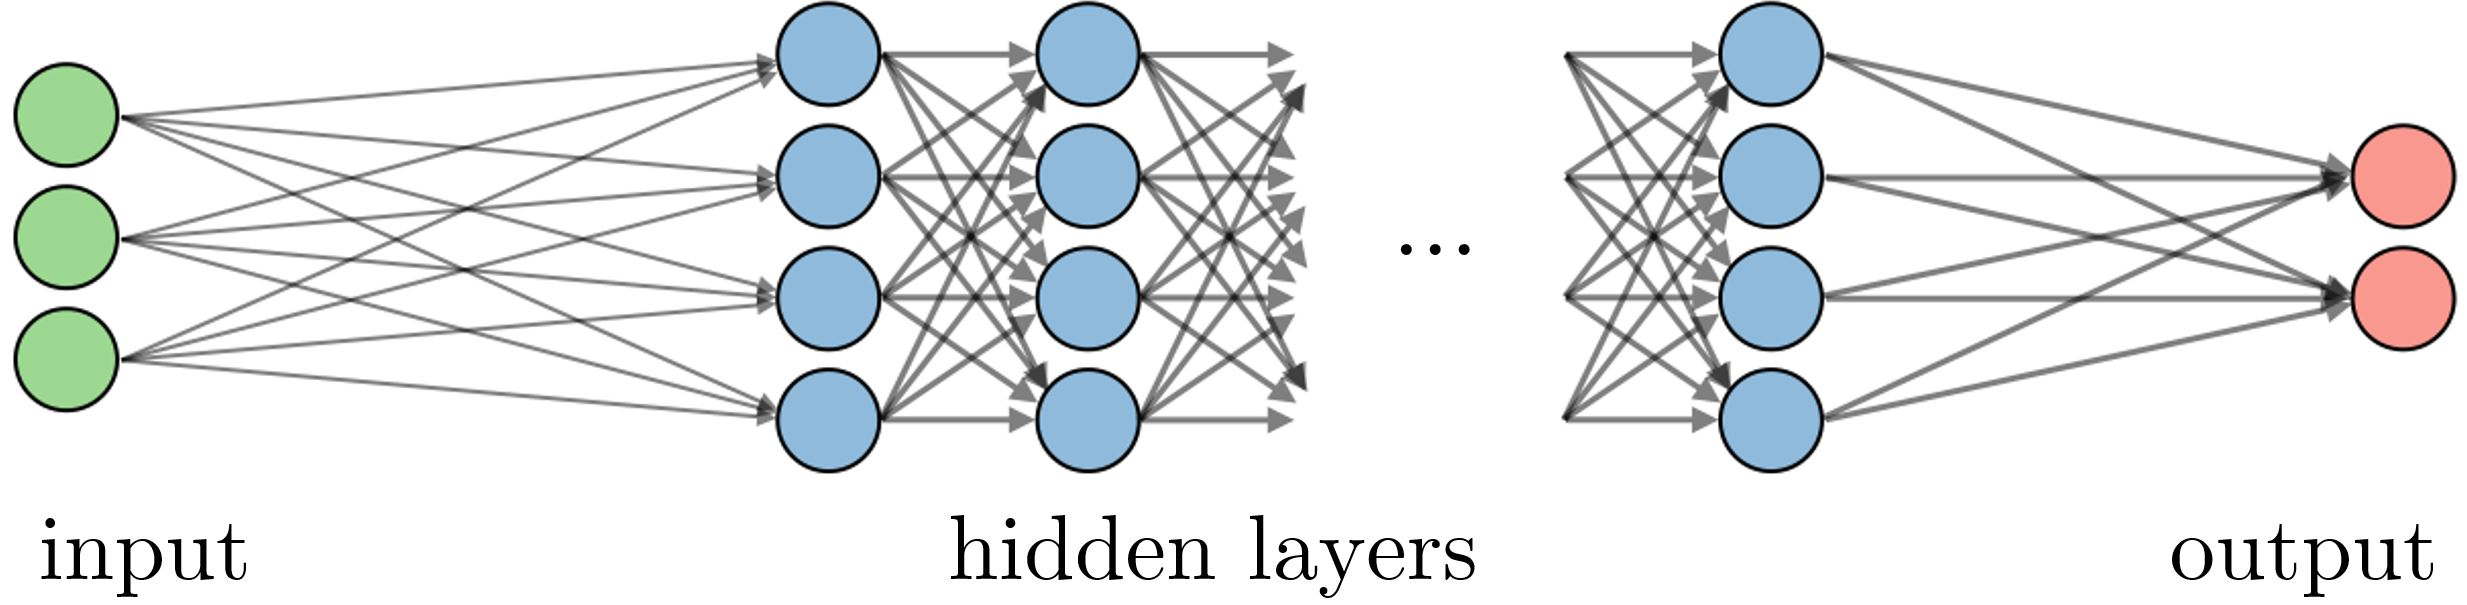
\includegraphics[width=\textwidth]{figures/nn3.JPG}
    \end{minipage}
\end{center}


\vspace{-5pt}
$\rightarrow$ \textbf{Input Layer}: The first layer that receives the input data. Each neuron in this layer corresponds to a \textbf{feature} of the input data. 

$\rightarrow$ \textbf{Hidden Layers}: Layers between the input and output layers where the network learn complex patterns.

$\rightarrow$ \textbf{Output Layer}: The final layer that produces the network's output, such as a prediction or classification.

$\bullet$ \textbf{Perceptron} - the foundation of a neural network, and it is a single-layer neural network. An Artificial Neuron is a basic building block of a neural network. \\

$\bullet$ \textbf{Neural Network} - a multi-layer \textbf{perceptron} 

\vspace{-5pt}
\begin{center}
    \begin{minipage}{0.6\linewidth}
    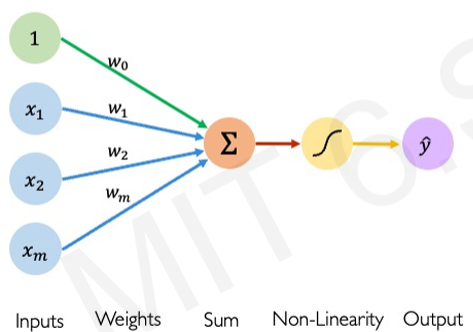
\includegraphics[width=\textwidth]{figures/perceptron_artificial_neuron.png}
    \end{minipage}
\end{center}


\vspace{-7pt}
\begin{center}
    \begin{minipage}{0.5\linewidth}
    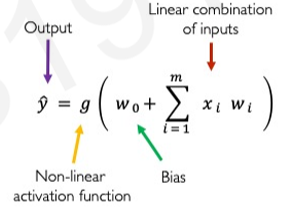
\includegraphics[width=\textwidth]{figures/perceptron_artificial_neuron_equation.png}
    \end{minipage}
\end{center}
\vspace{-5pt}





$\rightarrow$ \textbf{Weights}: are the real values that are attached with each input/feature and they convey the importance of that feature in predicting the final output. \\
$\rightarrow$ \textbf{Bias}: is used for shifting the activation function towards left or right.\\
$\rightarrow$ \textbf{Summation Function}: used to bind the weights and inputs together and calculate their sum. \\
$\rightarrow$ \textbf{Activation Function}: decides whether a neuron should be activated or not, and it introduces \textbf{non-linearities} into the network which makes input capable of learning and performing more complex tasks. 

\vspace{-5pt}
\begin{center}
    \begin{minipage}{\linewidth}
    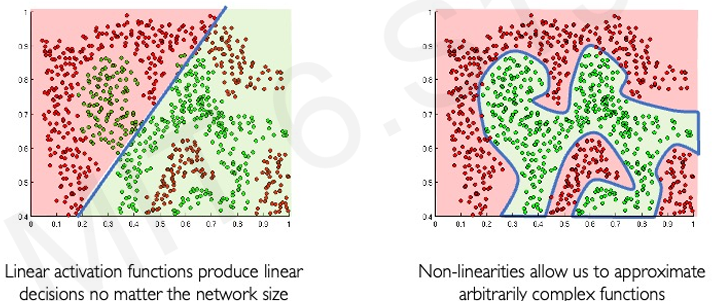
\includegraphics[width=\textwidth]{figures/activation_function_need.png}
    \end{minipage}
\end{center}
\vspace{-5pt}


\vspace{-1mm}
\begin{center}
\begin{tabular}{c|c|c}
          Sigmoid & ReLU & Tanh\\
         \hline
         \rule{0pt}{3ex}
         $\frac{1}{1+e^{-z}} $  & max$(0,z)$ & $\frac{e^z - e^{-z}}{e^z + e^{-z}}$\\
           &   &  \vspace{-2mm}\\

         \hline
         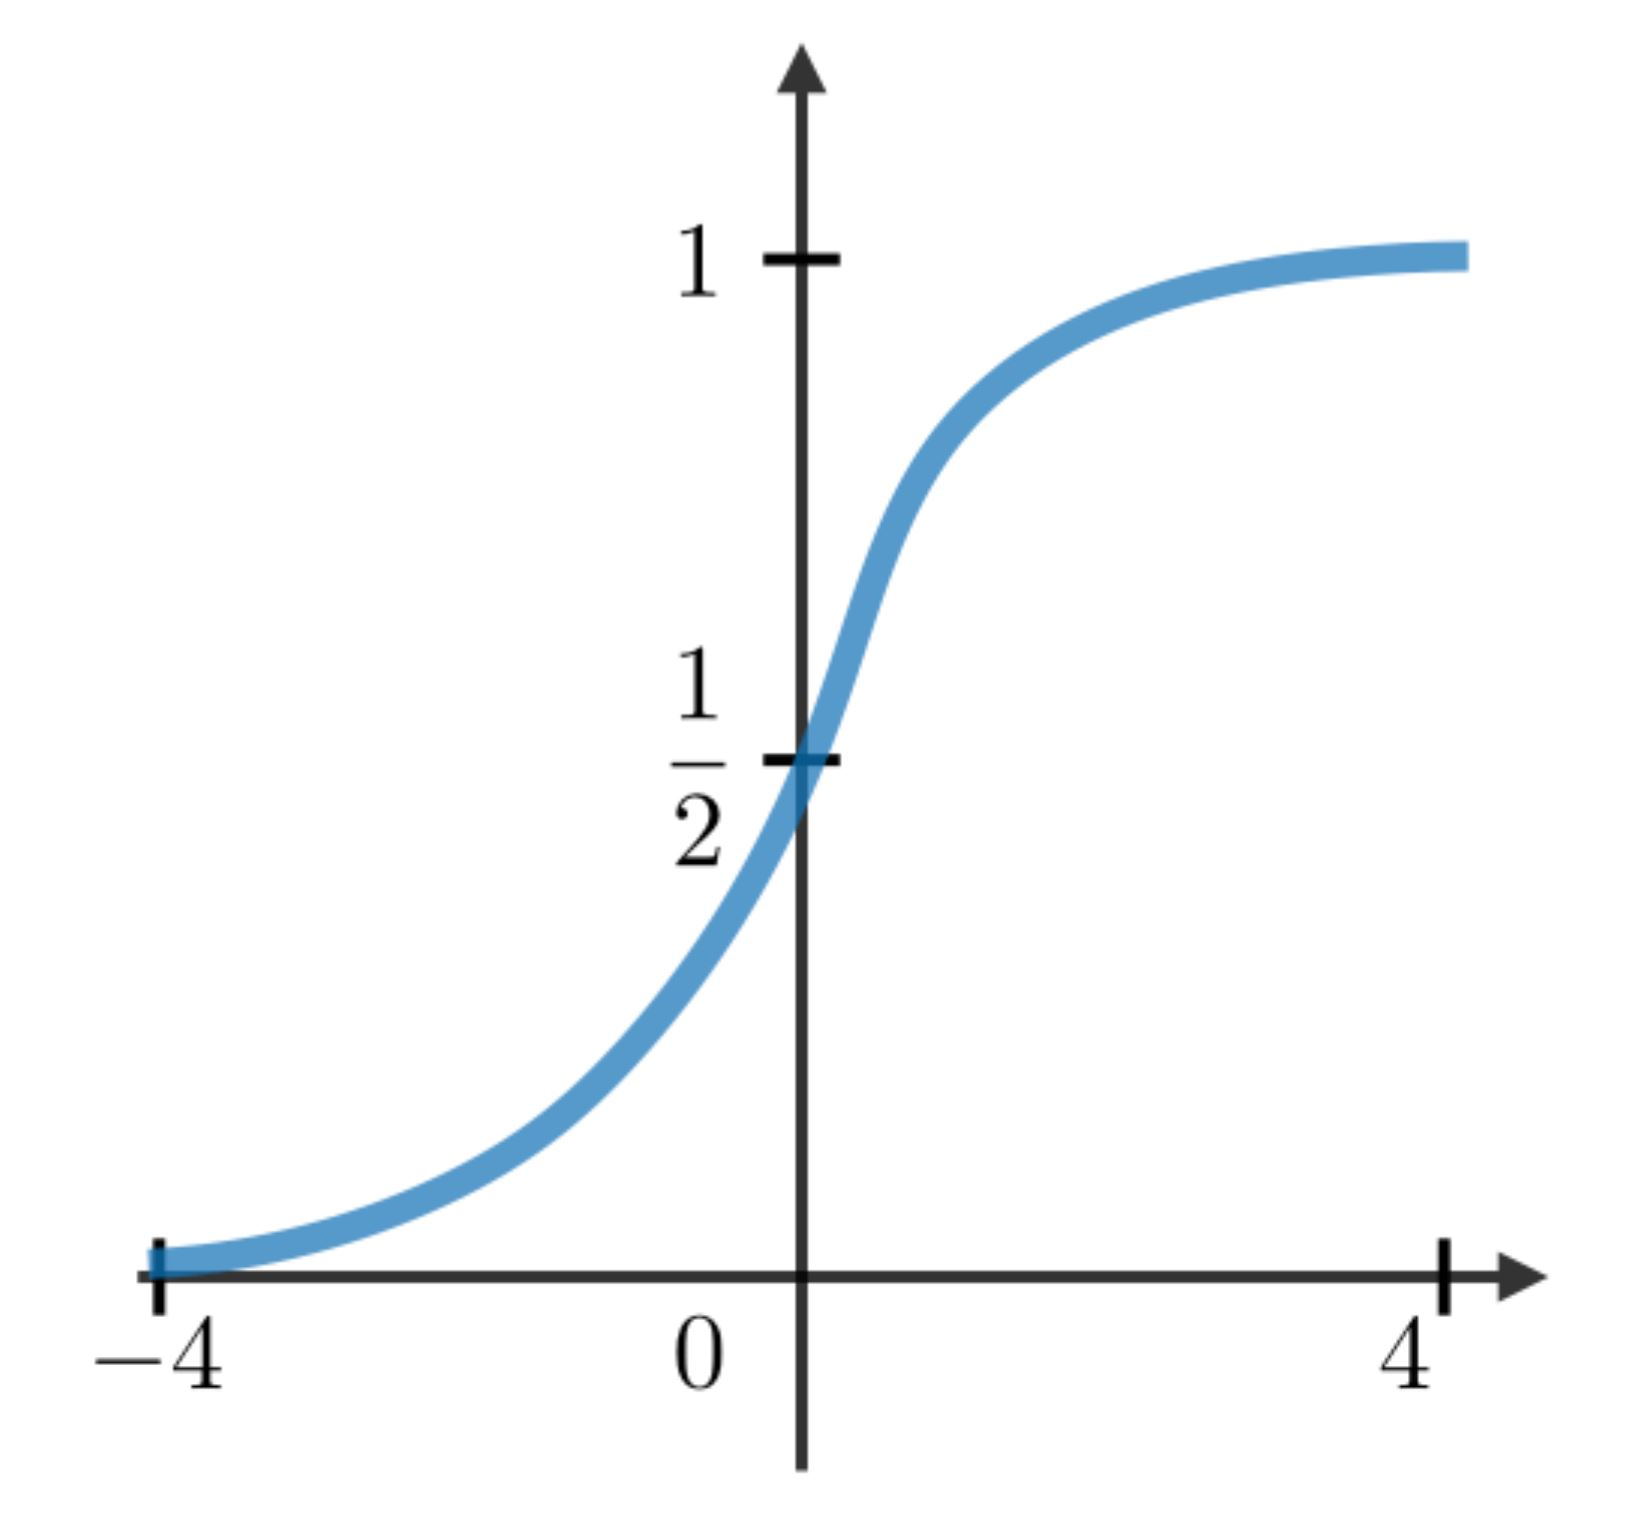
\includegraphics[scale = .047]{figures/sigmoid1.JPG} &
         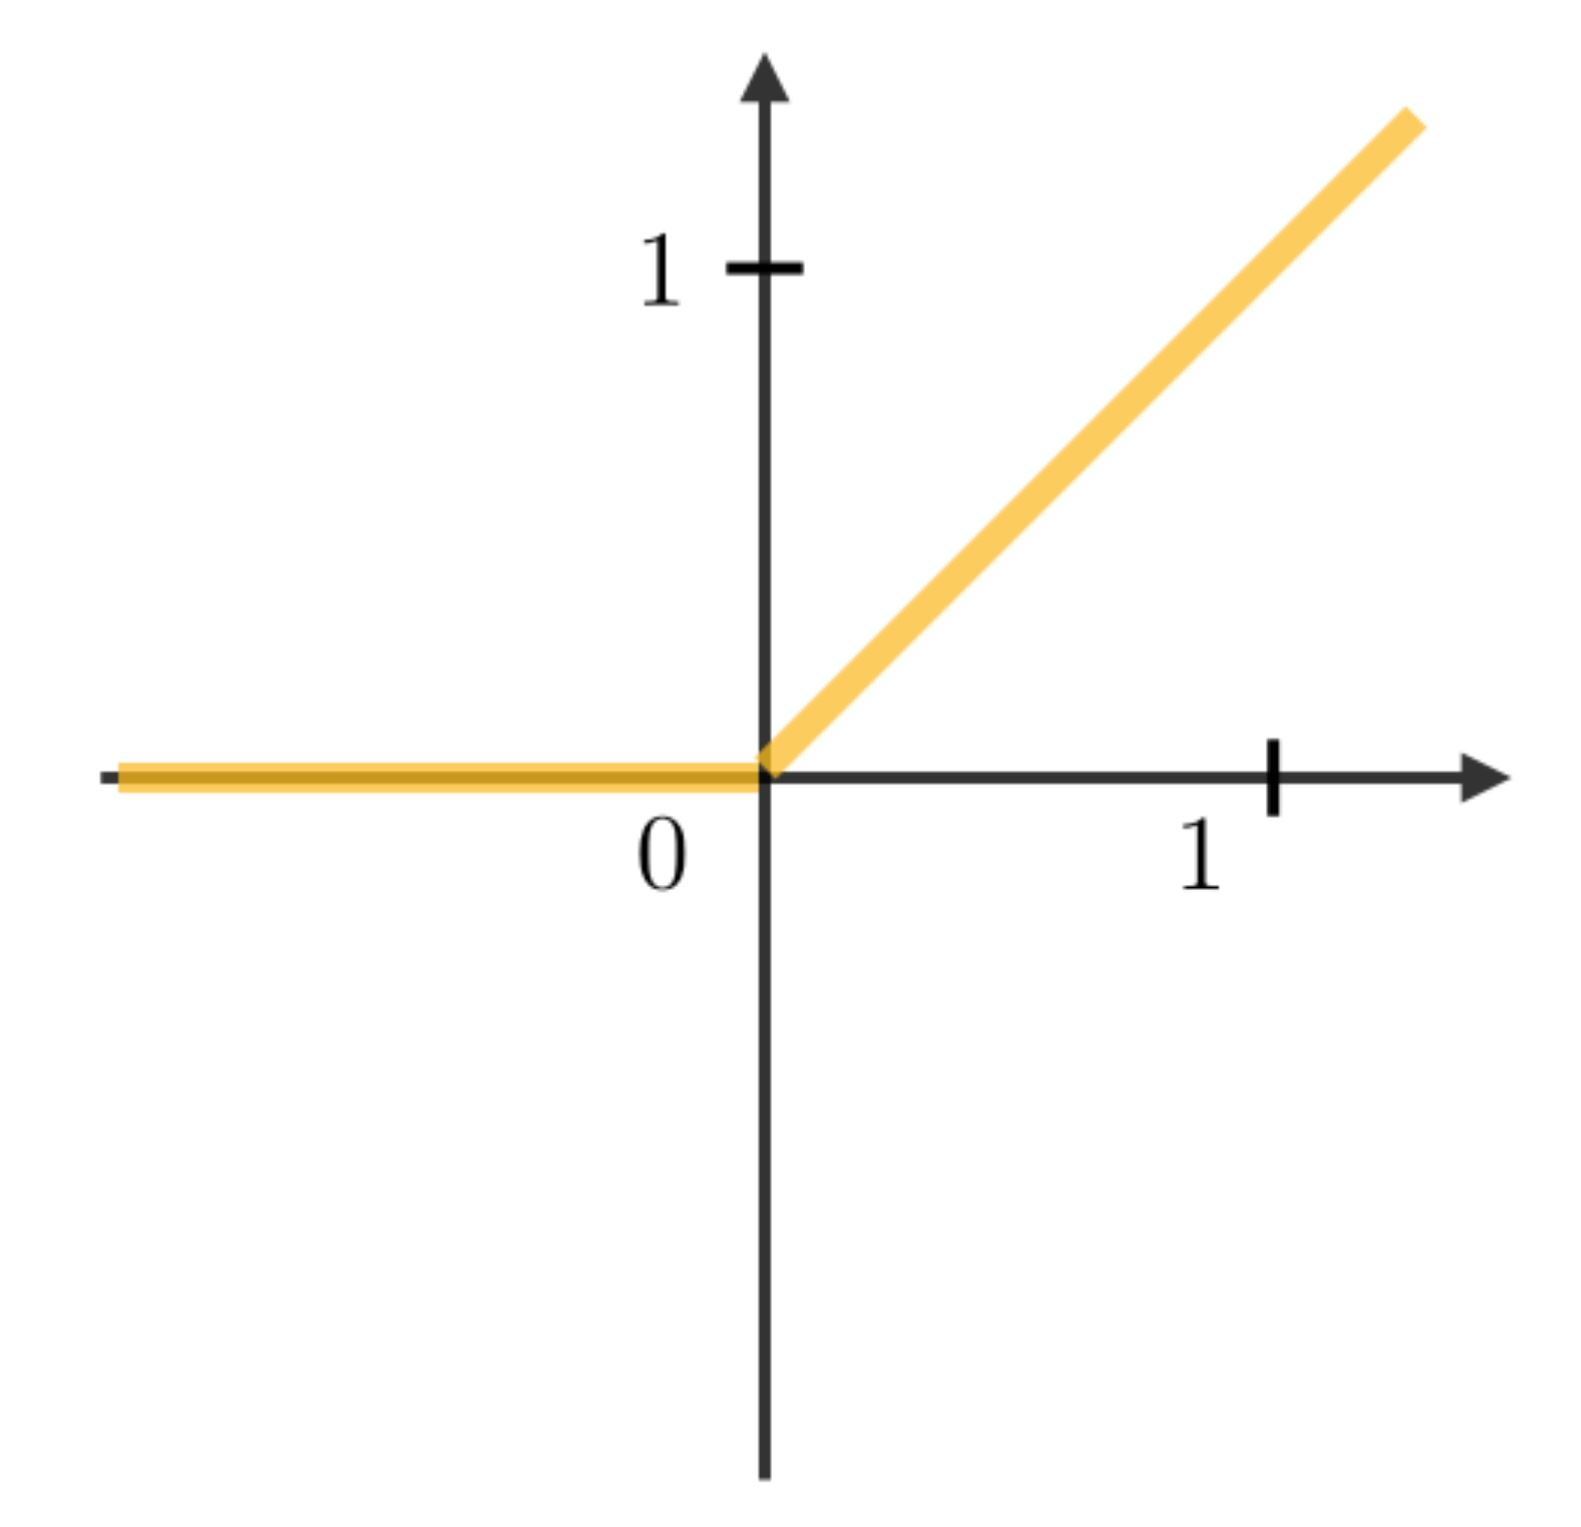
\includegraphics[scale = .047]{figures/relu.JPG} &
         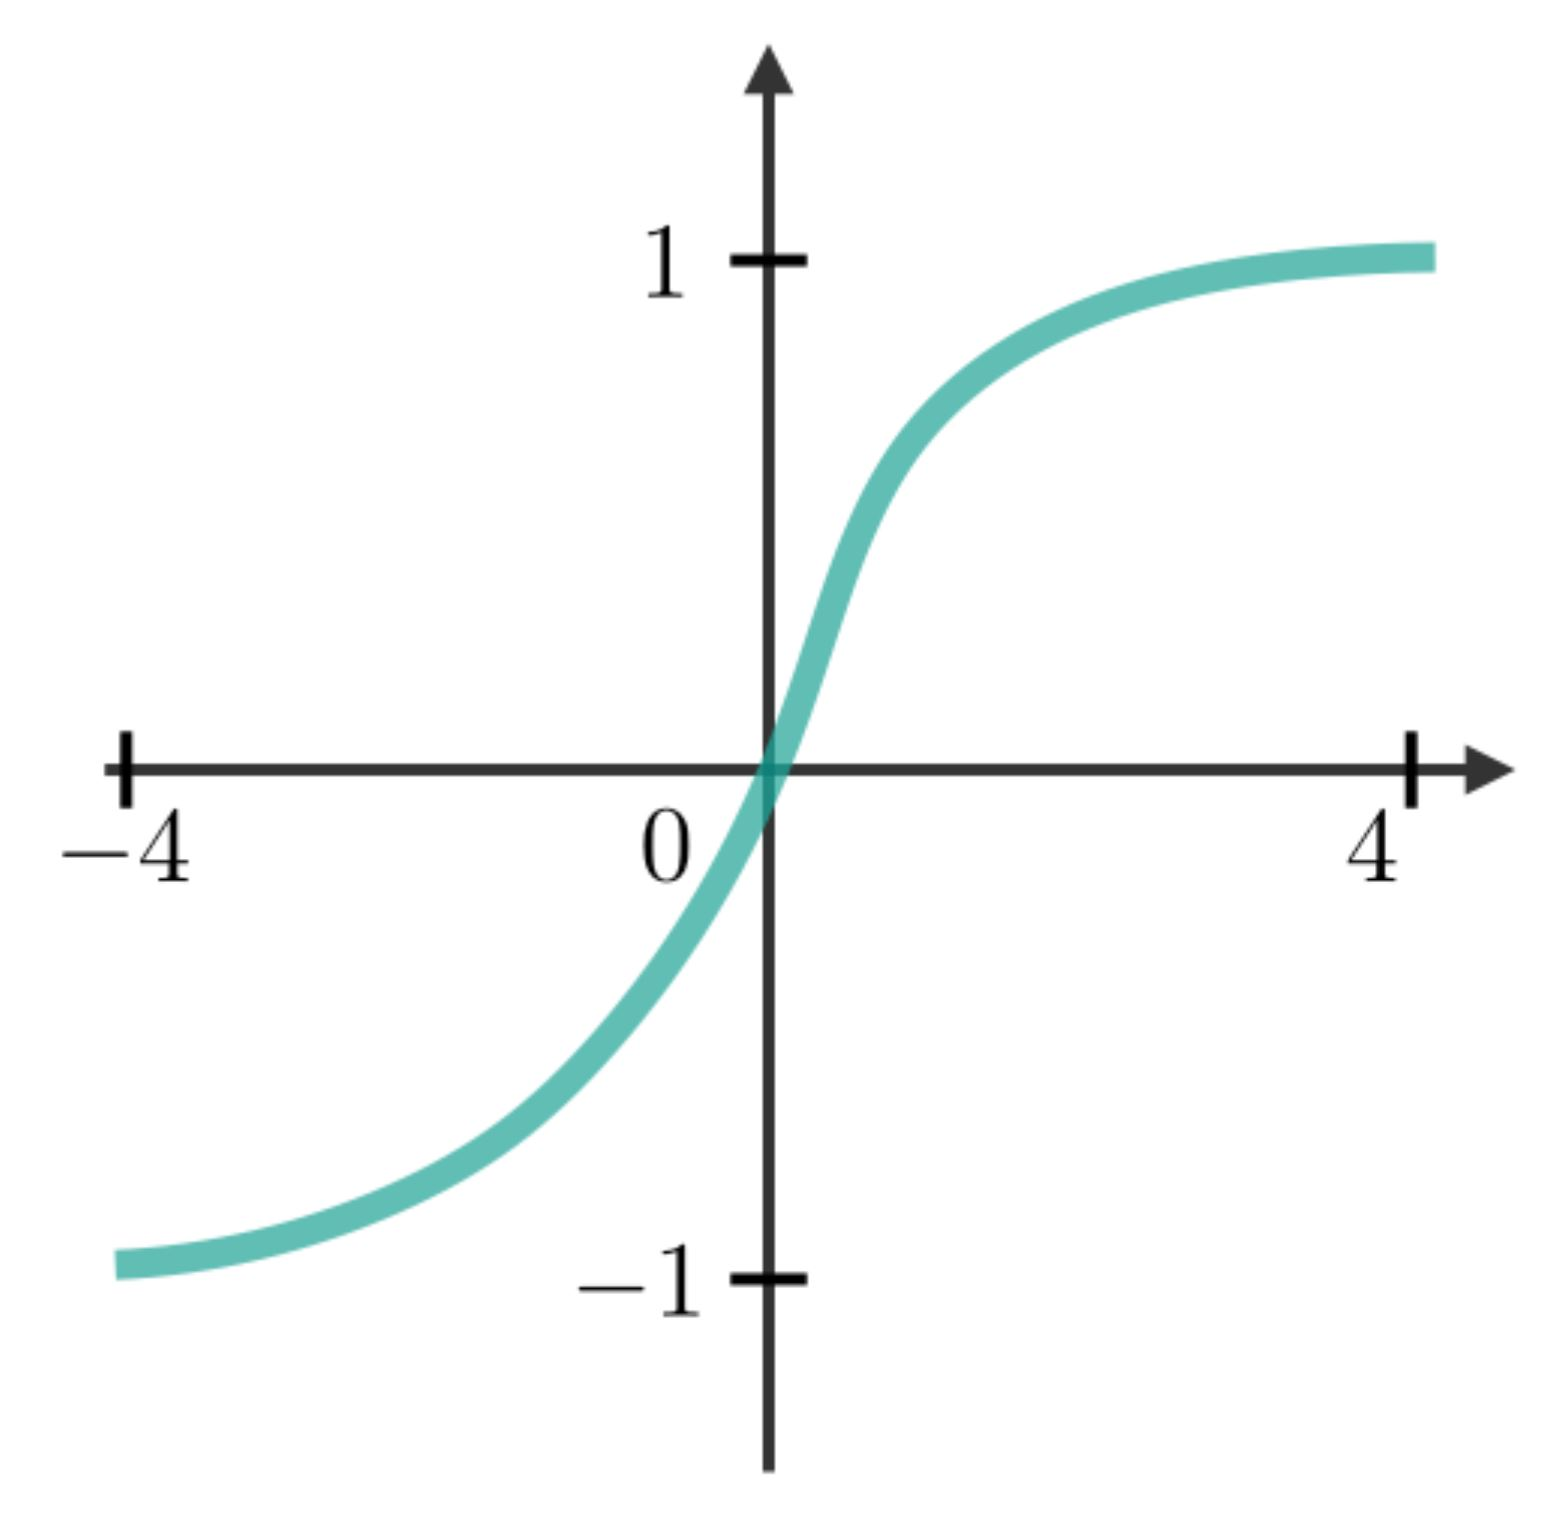
\includegraphics[scale = .047]{figures/tanh.JPG}

\end{tabular}
\end{center}






$\rightarrow$ \textbf{Softmax} - used as the last activation function of a neural network to normalize the output of a network to a probability distribution over predicted output classes. These probabilities sum to 1 $\to \frac{e^{z_i}}{\sum e^{z}}$

$\rightarrow$ If there is more than one `correct' label, the sigmoid function provides probabilities for all, some, or none of the labels.





\vspace{3pt}
\textbf{\textcolor{teal}{How Neural Networks Work?}} \\
$\bullet$  \textbf{Forward Propagation:} The input data is passed through the network, layer by layer, with each neuron applying its weights and bias to the input and passing the result through the activation function. The final layer produces the output.

\vspace{2pt}

$\bullet$ \textbf{Backpropagation:} Backpropagation is an algorithm used in neural networks to adjust the internal weights and biases to minimize the error calculated by the loss function. 
\vspace{-3pt}
\begin{itemize}[label={--},leftmargin=4mm]
\item \textbf{Regression Loss}: Mean Squared Error/Squared loss/ L2 loss, Mean Absolute Error/ L1 loss, Huber Loss 
\vspace{-3pt}
\item \textbf{Classification Loss}: Binary Cross Entropy/log loss, Categorical Cross Entropy
\vspace{-3pt}
\end{itemize}
The common loss functions are summed up in the table below:
\vspace{-5pt}
\begin{center}
    \begin{tabular}{c|c|c}
            \textbf{Least squared error} & \textbf{Logistic loss} & \textbf{Hinge loss} \\
            \hline
             $\frac{1}{2}(y-\hat{y})^{2}$ & $\text{log}\left(1+\text{exp}(-y\hat{y})\right)$ & $\text{max}(0, 1-y\hat{y})$  \\
            \hline 
            Linear Regression & Logistic Regression & SVM \\
            \hline
            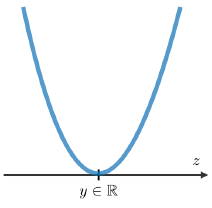
\includegraphics[scale = 0.4]{figures/least_squared_loss_func.PNG} &
            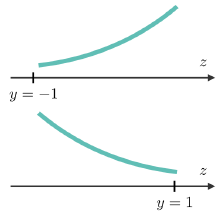
\includegraphics[scale = 0.4]{figures/logistic_loss_func.PNG} &
            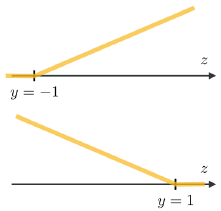
\includegraphics[scale = 0.4]{figures/hinge_loss_func.PNG}
    \end{tabular}
\end{center}



\vspace{2pt}
$\rightarrow$ During training, the network uses a supervised learning method where the difference (error) between the network's predicted output and the known expected output is calculated. This error is then propagated back through the network via backpropagation to compute the gradient of the loss function with respect to each weight. An optimization algorithm, such as gradient descent, uses these gradients to update the weights and biases, reducing the error and improving the model's accuracy over time.





\vspace{2pt}
$\bullet$ \textbf{Training:} The process of forward propagation, loss calculation, and backpropagation is repeated over many iterations, allowing the network to learn from the data and improve its accuracy.

$\bullet$ To prevent \textbf{overfitting}, regularization can be applied by:
\vspace{-3pt}
\begin{itemize}[label={--},leftmargin=6mm]
\itemsep -.4mm
\item Stopping training when validation performance drops
\item \textbf{Dropout} - randomly drop some nodes during training to prevent over-reliance on a single node
\item Embedding weight penalties into the objective function
\item \textbf{Batch Normalization} - stabilizes learning by normalizing inputs to a layer
\end{itemize}




\vspace{-5pt}

\begin{center}
    \begin{minipage}{\linewidth}
    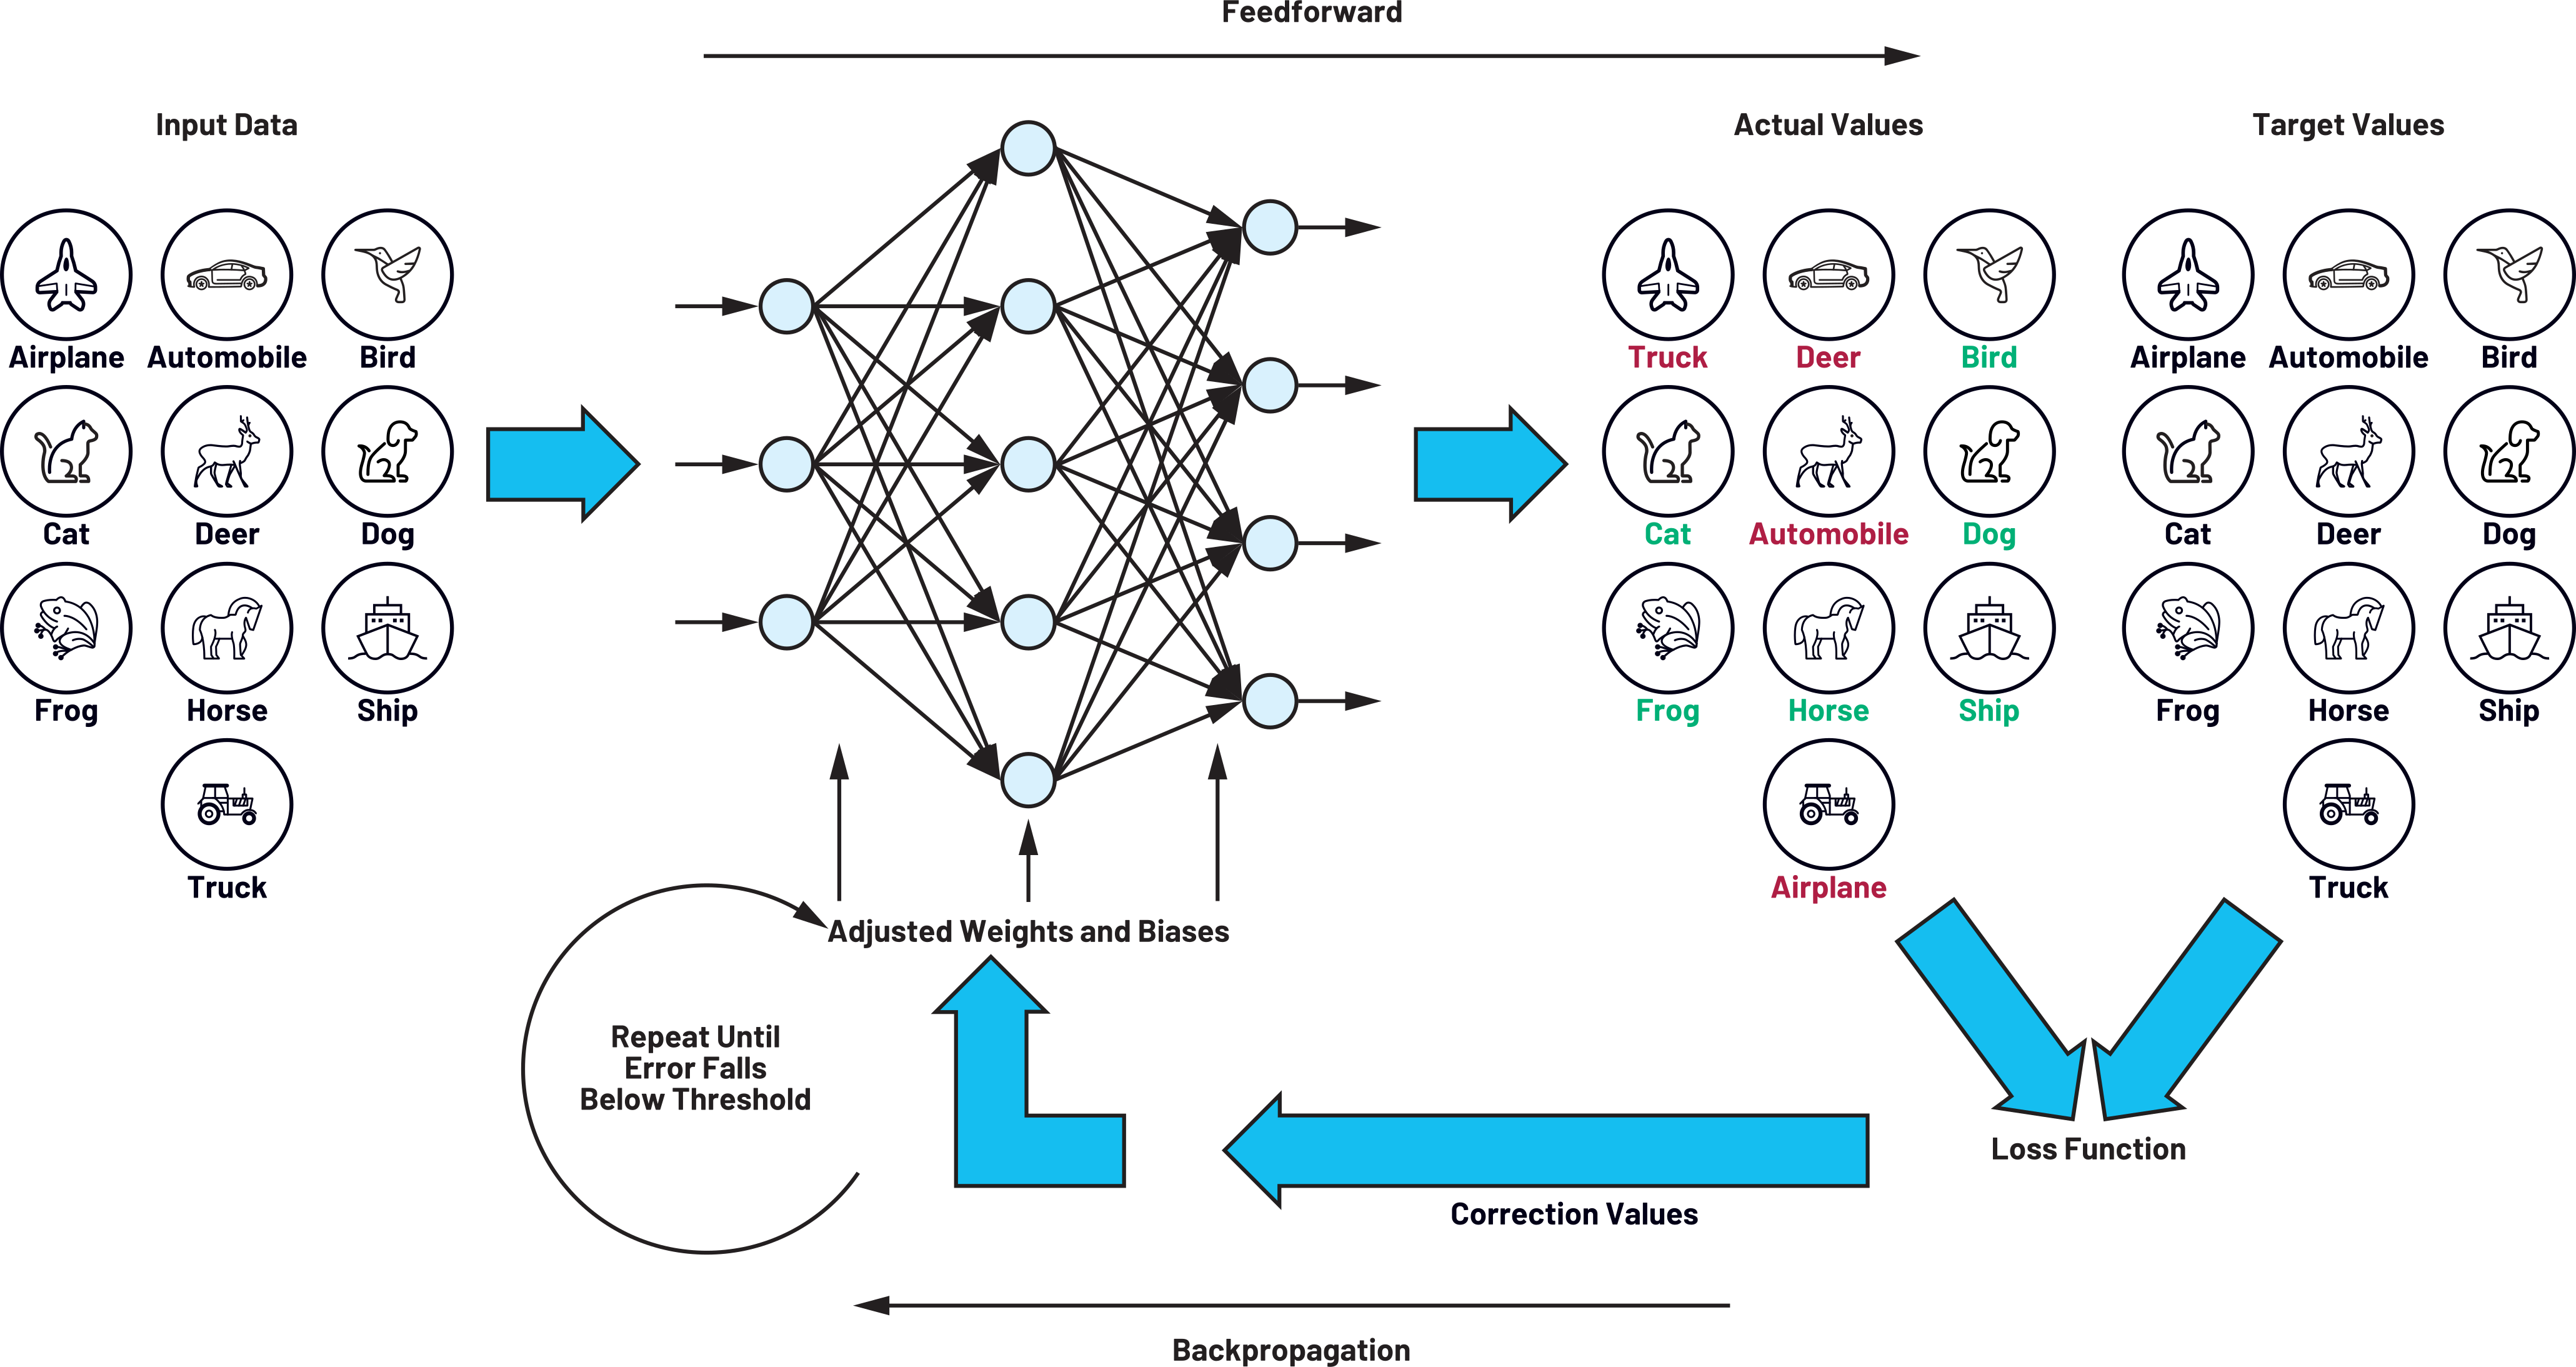
\includegraphics[width=\textwidth]{figures/feedforward_backpropagation.png}
    \end{minipage}
\end{center}

\vspace{-5pt}





%%%%%%%%%%%%%%%%% Convolutional Network %%%%%%%%%%%%%%%%%%%%%%%%%%
\section{Convolutional Neural Network} {\color{teal}\hrule height 1pt} \smallskip
CNN is a neural network architecture that is well-suited for image classification and object recognition tasks. The general CNN architectures are as shown below:
\vspace{-7pt}

\begin{center}
    \begin{minipage}{\linewidth}
    \includegraphics[width=\textwidth]{figures/cnn_architecture.png}
    \end{minipage}
\end{center}

\vspace{-7pt}

$\rightarrow$ A convolutional neural network starts by taking an input image, represented as a matrix of pixel values 

$\rightarrow$ This input image is passed through \textbf{convolutional layers}. Here, a set of filters applies to the input image to detect features like edges, textures, and patterns. Each filter produces a feature map that highlights a specific aspect of the input image. 

$\rightarrow$ After each convolution, an \textbf{activation function} (like ReLU) is applied to introduce non-linearity, enabling the network to learn more complex patterns.

$\rightarrow$ This produces \textbf{feature maps}. Different weights lead to different feature maps.
\vspace{-7pt}
\begin{center}
    \includegraphics[scale = .09]{figures/windowCNNNew.JPG}
\end{center}
\vspace{-7pt}

$\rightarrow$ The feature maps are then passed through \textbf{pooling layers}, which downsample the spatial dimensions by taking the maximum or average value in small regions. This reduces the size of the feature maps and retains essential information, making the network more efficient and less sensitive to slight changes in the input.

$\rightarrow$ Again, the \textbf{feature maps} produced by the convolutional layer and pooling layer are then passed through multiple additional convolutional and pooling layers, each layer learning increasingly complex features of the input image. 


$\rightarrow$ Now, the output obtained from above is fed into a \textbf{fully connected layer} for classification, object detection, or other structural analyses. The final output of the network is a predicted class label or probability score for each class, depending on the task.


\vspace{3pt}
\textbf{\textcolor{blue}{Question}}: Describe the difference between \textbf{batch normalization} and \textbf{layer normalization}.


\vspace*{\fill}

\columnbreak




%%%%%%%%%%%%%%%%%%%%%%% Recurrent Neural Network %%%%%%%%%%%%%%%%%%%%%%%%%
\section{Recurrent Neural Network} {\color{teal}\hrule height 1pt} \smallskip


Recurrent Neural Networks (RNNs) are designed to process sequences of data such as time series data, voice, natural language, and other activities.





\vspace{-5pt}

\begin{center}
    \begin{minipage}{0.75\linewidth}
    \includegraphics[width=\textwidth]{figures/RNNLoop.png}
    \end{minipage}
\end{center}
\vspace{-5pt}


$\rightarrow$ RNN memorize information from previous data with feedback loops inside it which helps to keep data information over time.


$\rightarrow$ It has an arrow pointing to itself, indicating that the data inside block “A” will be recursively used. Once expanded, its structure is equivalent to a chain-like structure. 

$\rightarrow$ Learning to store information or data over long periods of time intervals via recurrent backpropagation takes a very long time. Hence, the gradient gradually vanishes as they propagate to earlier time steps. These downstream gradients relies on parameter (weight) sharing for efficiency, and repeatedly multiplying values greater than or less than 1 leads to:

\begin{itemize}[label={--},leftmargin=4mm]
\vspace{-3pt}
\item \textbf{Exploding gradients} - model instability and overflows
\vspace{-3pt}
\item \textbf{Vanishing gradients} - loss of learning ability
\end{itemize}


$\rightarrow$ This can be solved using:
\begin{itemize}[label={--},leftmargin=4mm]
\vspace{-3pt}
\item \textbf{Gradient clipping} - cap the maximum value of gradients
\vspace{-3pt}
\item \textbf{ReLU} - its derivative prevents gradient shrinkage for $x > 0$
\vspace{-3pt}
\item \textbf{Gated cells} - regulate the flow of information
\end{itemize}

\vspace{3pt}

And, also for the non-convex problem, the RNN model training confuse between local minimum and global minimum. To overcome these problem, LSTM has been introduced as RNN languages modelling learning algorithm based on the feedforward architecture.

\vspace{-5pt}

\begin{center}
    \begin{minipage}{0.75\linewidth}
    \includegraphics[width=\textwidth]{figures/RNNBackprop.png}
    \end{minipage}
\end{center}

\vspace{-5pt}
$\bullet$ Vanishing gradient problem for RNNs. The sensitivity increases as the network backpropagates through in time. The darker the shade, the greater the sensitivity.
\vspace{-5pt}

\begin{center}
    \begin{minipage}{0.75\linewidth}
    \includegraphics[width=\textwidth]{figures/LSTMBackprop.png}
    \end{minipage}
\end{center}
\vspace{-5pt}
$\bullet$ Preservation of gradient information by LSTM. The sensitivity of the output layer can be switched on and off.

\vspace{2pt}


% \textbf{Long Short-Term Memory} - learns long-term dependencies using gated cells and maintains a separate cell state from what is outputted. Gates in LSTM perform the following:

% \begin{enumerate}[leftmargin=5mm]
% \itemsep -.4mm
% \item Forget and filter out irrelevant info from previous layers
% \item Store relevant info from current input
% \item Update the current cell state
% \item Output the hidden state, a filtered version of the cell state
% \end{enumerate}
% LSTMs can be stacked to improve performance.


% \vspace{3pt}
% LSTM is based on RNN, therefore, the basic structure of RNN is explained first and then LSTM structure is explained referencing RNN. 
% \vspace{-5pt}

% \begin{center}
%     \begin{minipage}{0.75\linewidth}
%     \includegraphics[width=\textwidth]{figures/RNNLoop.png}
%     \end{minipage}
% \end{center}
% \vspace{-5pt}



% LSTM memorize the information for the long period of time, which is important in many applications such as time prediction of the High frequency (HF) spectrum. The basic structure of the RNN and LSTM are similar as shown respectively below.


% \vspace{-5pt}

% \begin{center}
%     \begin{minipage}{0.75\linewidth}
%     \includegraphics[width=\textwidth]{figures/LSTMCell.png}
%     \end{minipage}
% \end{center}
% \vspace{-5pt}




$\rightarrow$ LSTM memorize the information for the long period of time. The difference between RNN and LSTM are: RNN cell has only \textbf{one} $\tanh$ layer while LSTM cell has \textbf{four} layers: forget gate layer, store gate layer, new cell state layer, output layer, and previous cell state as shown in Figure below.

% $\rightarrow$ The forget layer is responsible for deciding what information to retain from the previous cell state, and what information is to be forgotten or removed 
% \[f_{t} = \sigma(W_{t}.[h_{t-1},x_{t}] + b_{f}) \]


% $\rightarrow$ The store gate layer has an input gate using which we calculate another variable called new candidate values. The new candidate values are information which seem relevant are added to the cell state.
% \[i_{t} = \sigma(W_{i}.[h_{t-1},x_{t}] + b_{i})\]
% \[\Tilde{C}_{t} = \tanh(W_{c}.[h_{t-1},x_{t}] + b_{c})\]


% $\rightarrow$ The new cell state layer calculates the new cell state by updating the information from last cell. And the new cell state is calculated using the information acquired from the previous two layers.
% \[{C}_{t} = f_{t}*C_{t-1} + i_{t}*\Tilde{C_{t}}\]


% $\rightarrow$ The output layer makes use of all this information gathered over the last three layers to produce an output.
% \[o_{t} = \sigma(W_{o}.[h_{t-1},x_{t}] + b_{o})\]
% \[h_{t} = o_{t}*\tanh(C_{t})\]


% $\rightarrow$ Also, the cell state at the top of the Figure starting with $c({t-1})$ runs horizontally as it keeps the information integrity from long period of time with some minor linear attractions.  









%%%%%%%%%%%%%%%%% Time Series Analysis %%%%%%%%%%%%%%%%%%%%%%%
\section{Time Series} {\color{teal}\hrule height 1pt} \smallskip
Time Series is generally data which is collected over time and is dependent on it.

\vspace{2pt}

It is a random sequence $\{X_{t} \}$ of real values recorded at successive equally spaced points in time. \\

$\rightarrow$ Not every data collected with respect to time represents a time series. \\
$\rightarrow$ Methods of prediction \& forecasting, time based data is Time Series Modeling \\

\vspace{2pt}
$\bullet$ \textbf{Examples} of time series: Stock Market Price, Passenger Count of airlines, Temperature over time, Monthly Sales Data, Quarterly/Annual Revenue, Hourly Weather Data/Wind Speed, IOT sensors in Industries and Smart Devices, Energy Forecasting

\vspace{3pt}
$\rightarrow$ Difference between \textbf{Time Series} and \textbf{Regression} \\
$\bullet$ \textbf{Time Series} is time dependent. However the basic assumption of a linear regression model is that the observations are independent. \\
$\bullet$ Along with an increasing or decreasing trend, most Time Series have some form of seasonality trends\\

\vspace{3pt}
\textcolor{blue}{\textbf{Note}:}\\
$\rightarrow$ Predicting a time series using regression techniques is not a good approach. \\
$\rightarrow$ Time series forecasting is the use of a model to predict future values based on previously observed values.


\vspace{5pt}
$\rightarrow$ A stochastic process is defined as a collection of random variables $X=\{X_{t} \hspace{2pt}: t \in T\}$ defined on a common probability space, taking values in a common set $S$ (the state space), and indexed by a set $T$, often either $N$ or $[0, \infty)$ and thought of as time (discrete or continuous respectively) (Oliver, 2009).



\subsection{Time Series Statistical Models} {\color{teal}\hrule height 0.5pt} \smallskip

A \textbf{time series model} specifies the joint distribution of the sequence $\{X_{t} \}$ of random variables; e.g., 
\vspace{-3pt}
\[P\left(X_{1} \leq x_{1}, \ldots, X_{t} \leq x_{t}\right) \hspace{3pt} \text{for all} \hspace{3pt} t \hspace{3pt} \text{and} \hspace{3pt} x_{1},\ldots, x_{t} \]

Typically, a time series model can be described as 
\vspace{-3pt}
\[X_{t} = m_{t} + s_{t} + Y_{t} \]

where $m_{t}$: trend component; $s_{t}$: seasonal component; $Y_{t}$: Zero-mean error 

\vspace{3pt}
\textcolor{blue}{Note:} The following are some zero-mean models \\

$\rightarrow$ \textbf{iid noise}: The simplest time series model is the one with no trend or seasonal component, and the observations $X_{t}$s are simply independent and identically distribution random variables with zero mean. Such a sequence of random variable $\{X_{t}\}$ is referred to as \textbf{iid noise}.
\vspace{-3pt}
\[P\left(X_{1} \leq x_{1}, \ldots, X_{t} \leq x_{t} \right) = \prod_{t} P \left(X_{t} \leq x_{t}\right) = \prod_{t} F(x_{t})\] where $F(\cdot)$ is the cdf of each $X_{t}$. Further $E(X_{t}) = 0$ for all $t$. We denote such sequence as $X_{t} \sim \text{IID}(0, \sigma^{2})$. IID noise is not interesting for forecasting since $X_{t}|X_{1}, \ldots, X_{t-1} = X_{t}$. \\

$\rightarrow$ \textbf{iid noise} example: A \textbf{binary (discrete) process} $\{X_{t} \}$ is a sequence of iid random variables $X_{t}$s with 
\vspace{-3pt}
\[P(X_{t} = 1) = 0.5, \hspace{5pt} P(X_{t} = -1) = 0.5 \]

\vspace{3pt}
$\rightarrow$ \textbf{Gaussian Noise} example:A \textbf{continues process}: Gaussian noise $\{X_{t}\}$ is a sequence of iid normal random variables with zero mean and $\sigma^{2}$ variance; i.e., \(X_{t} \sim N (0, \sigma^{2})\) \\


\vspace{3pt}
$\rightarrow$ \textbf{Random walk}: The random walk $\{S_{t}, t=0,1,2, \ldots \}$ (starting at zero, $S_{0} = 0$) is obtained by cumulatively summing (or "integrating") random variables; i.e., $S_{0}=0$ and $S_{t} = X_{1} + \cdots + X_{t}, \hspace{5pt} \text{for} \hspace{2pt} t=1,2,\ldots$ \\
where $\{X_{t} \}$ is iid noise with zero mean and $\sigma^{2}$ variance. Note that by differencing, we can recover $X_{t}$; i.e.,
\vspace{-3pt}
\[\nabla  S_{t} = S_{t} - S_{t-1} = X_{t} \]

\vspace{-3pt}
Further, we have
\vspace{-3pt}
\[E(S_{t}) =  E\left( \sum_{t} X_{t} \right) = \sum_{t} E(X_{t}) = \sum_{i} 0 = 0\]
\vspace{-3pt}
\[\text{Var}(S_{t}) = \text{Var}\left(\sum_{t} X_{t} \right) = \sum_{t} \text{Var}(X_{t}) = t\sigma^{2} \]


$\rightarrow$ \textbf{White Noise}: We say $\{X_{t} \}$ is a white noise; i.e., $X_{t} \sim \text{WN}(0, \sigma^{2})$, if $\{X_{t} \}$ is uncorrelated, i.e., $\text{Cov}\left(X_{t_{1}}, X_{t_{2}}\right) = 0 $ for any $t_{1}$ and $t_{2}$ with E$[X_{t}] = 0$ and $\text{Var}(X_{t} = \sigma^{2})$. \\

\vspace{3pt}
\textcolor{blue}{\textbf{Note:}} Every $\text{IID}(0, \sigma^{2})$ sequence is $\text{WN}(0, \sigma^{2})$ but not conversely. \\


\vspace{5pt}

$\bullet$ \textbf{Moving Average Smoother} This is an essentially non-parametric method for trend estimation. It takes averages of observations around $t$; i.e., it smooths the series. For example, let 
\vspace{-3pt}
\[X_{t} = \frac{1}{3}\left(W_{t-1} + W_{t} + W_{t+1} \right)\]
which is a three-point moving average of the white noise series $W_{t}$. 

\vspace{2pt}
$\rightarrow$ \textbf{AR(1)} model (\textbf{Autoregression} of order 1): Let
\vspace{-3pt}
\[X_{t} = 0.6X_{t-1} + W_{t} \]
where $W_{t}$ is a white noise series. It represents a regression or prediction of the current value $X_{t}$ of a time series as a function of the past two values of the series.




\subsection{Stationary Process} {\color{teal}\hrule height 0.5pt} \smallskip








Extracts characteristics from time-sequenced data, which may exhibit the following characteristics:
\begin{itemize}[label={--},leftmargin=4mm]
\vspace{-3pt}
\item \textbf{Stationarity} - statistical properties such as mean, variance, auto-correlation are constant over time, an autocovariance that does not depend on time, and no trend or seasonality
\vspace{-3pt}
\item \textbf{Non-Stationary} - There are 2 major reasons behind the non-stationary of a Time Series 
\vspace{-3pt}
    \begin{itemize}
        \vspace{-3pt}
        \item Trend - varying mean over time (mean is not constant)
        \vspace{-3pt}
        \item Seasonality - variations at specific time-frames (standard deviation is not constant)
    \end{itemize}
    
\item \textbf{Trend} - Trend is a general direction in which something is developing or changing.
\vspace{-3pt}
\item \textbf{Seasonality} - Any predictable change or pattern in a time series that recurs or repeats over a specific time period (calendar times) occurring at regular intervals less than a year
\vspace{-3pt}
\item \textbf{Cyclicality} - variations without a fixed time length, occurring in periods of greater or less than one year
\vspace{-3pt}
\item \textbf{Autocorrelation} - degree of linear similarity between current and lagged values
\end{itemize}


$\bullet$ CV must account for the time aspect, such as for each fold $F_x$:
\begin{itemize}[label={--},leftmargin=4mm]
\vspace{-3pt}
\item \textbf{Sliding Window} - train $F_1$, test $F_2$, then train $F_2$, test $F_3$
\vspace{-3pt}
\item \textbf{Forward Chain} - train $F_1$, test $F_2$, then train $F_1, F_2$, test $F_3$
\end{itemize}

$\bullet$ \textbf{Exponential Smoothing} - uses an exponentially decreasing weight to observations over time, and takes a moving average. The time $t$ output is $s_t = \alpha x_t + (1-\alpha)s_{t-1}$, where  $0 < \alpha < 1$.
\smallskip

$\bullet$ \textbf{Double Exponential Smoothing} - applies a recursive exponential filter to capture trends within a time series
    \begin{center}
    \vspace{-2.5mm}
    $s_t = \alpha x_t + (1-\alpha)(s_{t-1} + b_{t-1})$\\
    $b_t = \beta (s_t - s_{t-1}) + (1-\beta)b_{t-1}$\\
    \vspace{-2mm}
    \end{center}
Triple exponential smoothing adds a third variable
$\gamma$ that accounts for seasonality.
\smallskip

$\bullet$ \textbf{ARIMA} - models time series using three parameters $(p,d,q)$:

\begin{itemize}[label={--},leftmargin=4mm]
\vspace{-3pt}
\item \textbf{Autoregressive} - the past $p$ values affect the next value
\vspace{-3pt}
\item \textbf{Integrated} - values are replaced with the difference between current and previous values, using the difference degree $d$ (0 for stationary data, and 1 for non-stationary)
\vspace{-3pt}
\item \textbf{Moving Average} - the number of lagged forecast errors and the size of the moving average window $q$
\end{itemize}

$\bullet$ \textbf{SARIMA} - models seasonality through four additional seasonality-specific parameters: $P$, $D$, $Q$, and the season length $s$
\smallskip

$\bullet$ \textbf{Prophet} - additive model that uses non-linear trends to account for multiple seasonalities such as yearly, weekly, and daily. \\
$\rightarrow$ Robust to missing data and handles outliers well.\\ 
$\rightarrow$ Can be represented as: $y(t) = g(t) + s(t) + h(t) + \epsilon(t)$, with four distinct components for the growth over time, seasonality, holiday effects, and error. This specification is similar to a generalized additive model.
\smallskip

$\bullet$ \textbf{Generalized Additive Model} - combine predictive methods while preserving additivity across variables, in a form such as
$y = \beta_0 + f_1(x_1) + \cdots + f_m(x_m)$, where functions can be non-linear. \\
$\rightarrow$ GAMs also provide regularized and interpretable solutions for regression and classification problems.


\vspace{5pt}
\textcolor{blue}{\textbf{Tutorial}:} \href{https://www.kaggle.com/code/prashant111/complete-guide-on-time-series-analysis-in-python}{\textbf{Complete Guide on Time Series Analysis in Python}}




% \vspace*{\fill}

% \columnbreak

%%%%%%%%%%%%%%%%%%%%%%%% Natural Language Processing %%%%%%%%%%%%%%%%%%%%%%%%%%%%%%
\section{Natural Language Processing} {\color{teal}\hrule height 1pt} \smallskip


\textbf{NLP} is the discipline of building machines that can manipulate human language — or data that resembles human language — in the way that it is written, spoken, and organized. It evolved from computational linguistics.


\textbf{NLP Applications}
\vspace{-7pt}
\begin{center}
    \begin{minipage}{0.86\linewidth}
    \includegraphics[width=\textwidth]{figures/nlp_application.png}
    \end{minipage}
\end{center}
\vspace{-7pt}



\textbf{Evolution of NLP}
\vspace{-7pt}
\begin{center}
    \begin{minipage}{\linewidth}
    \includegraphics[width=\textwidth]{figures/nlp_evolution.png}
    \end{minipage}
\end{center}
\vspace{-7pt}

\textbf{Challenges in NLP}\\



\vspace{3pt}
$\bullet$ The 3 stages of an NLP pipeline are: Text Processing $\rightarrow$ Feature Extraction $\rightarrow$ Modeling.

\vspace{-7pt}
\begin{center}
    \begin{minipage}{0.9\linewidth}
    \includegraphics[width=\textwidth]{figures/three_stages_NLP.png}
    \end{minipage}
\end{center}
\vspace{-7pt}






\subsubsection{Text Processing} {\color{teal}\hrule height 0.5pt} \smallskip


Take raw input text, clean it, normalize it, and convert it into a form that is suitable for feature extraction. \\
\textbf{Libraries}: nltk, spacy


\begin{itemize}[label={--},leftmargin=4mm]
\vspace{-3pt}
\item \textbf{Lower casing}
\vspace{-3pt}

\item Removing other stuff like: punctuations, tags, URLs, etc depends on the problem
\vspace{-3pt}

\item Convert \textbf{chat words} used in social media to a normal word 
\vspace{-3pt}

\item Spelling correction using libraries like \textbf{TextBlob}
\vspace{-3pt}

\item \textbf{Stop words} - removes common and irrelevant words (\emph{the, is}) \\
\textbf{Note}: Do \textbf{not} remove stop words when using \textbf{POS Tagging} in text processing.
\vspace{-3pt}


\item \textbf{Tokenization} - splits text into individual words (tokens) and word fragments. \\
$\bullet$ \textbf{Sentence-level} tokenization involves splitting a text into individual sentences. \\
$\bullet$ \textbf{Word-level} tokenization involves splitting each sentence into individual words or tokens.
\vspace{-3pt}



\item \textbf{Lemmatization} - reduces words to its base form based on dictionary definition (\emph{am, are, is} $\to$ \emph{be})
\vspace{-3pt}

\item \textbf{Stemming} - reduces words to its base form without context (\emph{ended} $\to$ \emph{end})
\vspace{-3pt}

\item Language Detection
\vspace{-3pt}
\end{itemize}





\subsubsection{Advance Text Processing}  {\color{teal}\hrule height 0.5pt} \smallskip

\begin{itemize}[label={--},leftmargin=4mm]
\item \textbf{POS Tagging}


\vspace{-7pt}
\begin{center}
    \begin{minipage}{0.7\linewidth}
    \includegraphics[width=\textwidth]{figures/nlp_pos_tagging.png}
    \end{minipage}
\end{center}
\vspace{-7pt}

\item \textbf{Parse Tree}

\item \textbf{Coreference Resolution}


\end{itemize}


\subsubsection{Feature Extraction}  {\color{teal}\hrule height 0.5pt} \smallskip

$\rightarrow$ Feature Extraction = Text Representation =  Text Vectorization \\

\vspace{3pt}
\textbf{Common Terms}:\\
$\bullet$ Corpus
$\bullet$ Vocabulary
$\bullet$ Document
$\bullet$ Word


\vspace{-7pt}
\begin{center}
    \begin{minipage}{0.5\linewidth}
    \includegraphics[width=\textwidth]{figures/nlp_corpus_document_vocabulary.png}
    \end{minipage}
\end{center}
\vspace{-7pt}




$\rightarrow$ Most conventional machine learning techniques work on the features – generally numbers that describe a document in relation to the corpus that contains it – created by either Bag-of-Words, TF-IDF, or generic (custom) feature engineerings such as \textbf{document length}, \textbf{word polarity}, and metadata (for instance, if the text has associated \textbf{tags} or \textbf{scores}). \\

\vspace{3pt}
\textbf{Note}: Deep learning does \textbf{not} require to do \textbf{feature engineering} 

\begin{itemize}[label={--},leftmargin=4mm]

\item \textbf{Bag-of-words} - counts the number of times each word or $n$-gram (combination of n words) appears in a document.
\vspace{-3pt}


\vspace{-5pt}
\begin{center}
    \begin{minipage}{\linewidth}
    \includegraphics[width=\textwidth]{figures/tokenizers_bag_of_words.png}
    \end{minipage}
\end{center}
\vspace{-5pt}

\item $\boldsymbol{n}$\textbf{-gram} - predicts the next term in a sequence of $n$ terms based on Markov chains
\vspace{-3pt}


$\rightarrow$ \textbf{Markov Chain} - stochastic and memoryless process that predicts future events based only on the current state
\vspace{-3pt}


\vspace{-5pt}
\begin{center}
    \begin{minipage}{0.6\linewidth}
    \includegraphics[width=\textwidth]{figures/nlp_n_grams.png}
    \end{minipage}
\end{center}
\vspace{-5pt}


\item \textbf{tf-idf} - In contrast, with TF-IDF, we weight each word by its importance. To evaluate a word’s significance, we consider two things: 
\vspace{-3pt}
\begin{enumerate}
    \item \textbf{Term Frequency}: How important is the word in the document? 
    \(\text{TF(word in a document)} = \frac{\text{Number of occurrences of that word in document}}{\text{Number of words in document}}  \)
    \vspace{-3pt}
    \item \textbf{Inverse Document Frequency}: How important is the word in the whole corpus (a collection of documents)? \\
    \(\text{IDF(word in a corpus)} = \text{log} (\frac{\text{number of documents in the corpus}}{\text{number of documents that include the word}}) \)
    \vspace{-3pt}
\end{enumerate}

\textcolor{blue}{\textbf{Note}:} A word is important if it occurs many times in a document. But that creates a problem. Words like “a” and “the” appear often. And as such, their TF score will always be high. We resolve this issue by using Inverse Document Frequency, which is high if the word is rare and low if the word is common across the corpus. The TF-IDF score of a term is the product of TF and IDF. 


\textbf{Cosine Similarity} - measures similarity between vectors, calculated as cos($\theta$) =
$\frac{A\cdot B}{||A||||B||} $, which ranges from o to 1
\vspace{-3pt}

\vspace{-5pt}
\begin{center}
    \begin{minipage}{1\linewidth}
    \includegraphics[width=\textwidth]{figures/tokenizers_term_freq_TF_IDF.png}
    \end{minipage}
\end{center}
\vspace{-5pt}


\vspace{3pt}
$\rightarrow$ \textbf{CountVectorizer} - Bag of Words \\
$\rightarrow$ \textbf{TfidfTransformer} - TF-IDF values \\
$\rightarrow$ \textbf{TfidfVectorizer} - Bag of Words AND TF-IDF values \\



\end{itemize}








\subsubsection{Word Embedding}  {\color{teal}\hrule height 0.5pt} \smallskip

Word embeddings are often based on neural network models in deep learning. \\



$\rightarrow$ Based on CBOW, Skip gram: Word2vec, GloVe, fastText
\begin{itemize}[label={--},leftmargin=4mm]
\vspace{-3pt}
\item \textbf{Continuous bag-of-words} (CBOW) - predicts the word given its context
\vspace{-3pt}
\item \textbf{skip-gram} - predicts the context given a word
\end{itemize}


$\bullet$ \textbf{word2vec} - trains iteratively over a corpus of text to learn the association between the words, and preserve the \textbf{semantic} information as well as \textbf{contextual} meanings of words within a given corpus of text. \\

$\rightarrow$ They are numerical representations of words and phrases allowing \textbf{similar words} to have \textbf{similar vector} representations.\\


$\rightarrow$ It uses the cosine similarity metric to measure \textbf{semantic} similarity. If the cosine angle is one, it means that the words are overlapping. , such that $king - man + woman \approx queen$


\vspace{3pt}
\textbf{Note:} According to research \textbf{CBOW} is used when small dataset is available.

\vspace{-5pt}
\begin{center}
    \begin{minipage}{1\linewidth}
    \includegraphics[width=\textwidth]{figures/nlp_CBOW.png}
    \end{minipage}
\end{center}
\vspace{-5pt}



\vspace{3pt}
$\bullet$ \textbf{GloVe} (Global Vectors for Word Representation) - GloVe operates on the idea that words that frequently co-occur together, sharing similar contexts, tend to have related meanings. It builds a global co-occurrence matrix that captures the frequency of word co-occurrences within a context window across the entire corpus


\vspace{3pt}
$\rightarrow$ Based on transformer architecture  \\
$\bullet$ \textbf{BERT} - accounts for word order and trains on subwords, and unlike word2vec and GloVe, BERT outputs different vectors for different uses of words ($cell$ phone vs. blood $cell$)





\subsubsection{Sentiment Analysis}  {\color{teal}\hrule height 0.5pt} \smallskip
Extracts the attitudes and emotions from text

$\bullet$ \textbf{Polarity} - measures positive, negative, or neutral opinions
\begin{itemize}[label={--},leftmargin=4mm]
\vspace{-3pt}
\item Valence shifters - capture amplifiers or negators such as '$really$ fun' or '$hardly$ fun'
\end{itemize}


$\bullet$ \textbf{Sentiment} - measures emotional states such as happy or sad \\
$\bullet$ \textbf{Subject-Object Identification} - classifies sentences as either subjective or objective



\subsubsection{Topic Modelling}  {\color{teal}\hrule height 0.5pt} \smallskip
Captures the underlying themes that appear in documents\\
$\bullet$ \textbf{Latent Dirichlet Allocation} (LDA) - generates $k$ topics by first assigning each word to a random topic, then iteratively updating assignments based on parameters $\alpha$, the mix of topics per document, and $\beta$, the distribution of words per topic \\

$\bullet$ \textbf{Latent Semantic Analysis} (LSA) - identifies patterns using tf-idf scores and reduces data to $k$ dimensions through SVD

\vspace{10pt}

\href{https://www.youtube.com/watch?v=ruyyyRp79uQ&list=PLkz_y24mlSJarFAx94xU17AJ7QJNG1Erl}{\textbf{NLP Tutorial}}

\href{https://www.youtube.com/watch?v=1fvQU5yPjFs&list=PLKnIA16_RmvZo7fp5kkIth6nRTeQQsjfX&index=8}{Duplicate Question Pairs - Quora Questions Pairs: NLP Pipeline}



\vspace*{\fill}
\columnbreak

%%%%%%%%%%%%%%%%%%% Recommender System %%%%%%%%%%%%%%%%%%%%%%%%%%%%%%
\section{Recommender System} {\color{teal}\hrule height 1pt} \smallskip

The Recommender System utilizes machine learning and data analysis to provide personalized suggestions to users. \\
$\rightarrow$ It operates by collecting and analyzing user behavior, user preferences, and historical user-item interactions.

\vspace{3pt}

$\bullet$ Two main types of recommender system:
\vspace{-3pt}
\begin{itemize}[label={--},leftmargin=4mm]
\item \textbf{Collaborative Filtering} - recommends what similar users like
\vspace{-3pt}
\item \textbf{Content Filtering} - recommends similar items
\end{itemize}

\vspace{-5pt}
\begin{center}
    \begin{minipage}{\linewidth}
    \includegraphics[width=\textwidth]{figures/collaborative_content_recommender_system.png}
    \end{minipage}
\end{center}
\vspace{-5pt}



Collaborative filtering is more common and includes methods such as: \\
$\bullet$ \textbf{Memory-based Approaches} - finds neighborhoods by using \textbf{rating data} to compute user and item similarity, measured using correlation or cosine similarity

\begin{itemize}[label={--},leftmargin=4mm]
\vspace{-3pt}
\item \textbf{User-User} - similar users also liked...
\vspace{-3pt}
\begin{itemize}[label={--},leftmargin=4mm]
    \vspace{-3pt}
    \item Leads to more diverse recommendations, as opposed to just recommending popular items
    \vspace{-3pt}
    \item Suffers from sparsity, as the number of users who rate items is often low
    \end{itemize}
    \vspace{-1mm}
\item \textbf{Item-Item} - similar users who liked this item also liked...
    \vspace{-3pt}
    \begin{itemize}[label={--},leftmargin=4mm]
    \vspace{-3pt}
    \item Efficient when there are more users than items, since the item neighborhoods update less frequently than users
    \vspace{-3pt}
    \item Similarity between items is often more reliable than similarity between users
    \end{itemize}
\end{itemize}
\vspace{-1.5mm}
\smallskip


$\bullet$ \textbf{Model-based Approaches} - predict ratings of unrated items, through methods such as Bayesian networks, SVD, and clustering. Handles sparse data better than memory-based approaches.
\begin{itemize}[label={--},leftmargin=4mm]
\vspace{-3pt}
\item \textbf{Matrix Factorization} - decomposes the user-item rating matrix into two lower-dimensional matrices representing the users and items, each with $k$ latent factors
\end{itemize}



$\rightarrow$ Recommender systems can also be combined through ensemble methods to improve performance.


\vspace*{\fill}



%%%%%%%%%%%%%%%%%%%%%% \section{References} %%%%%%%%%%%%%%%%%%%%%%%%%%%%%%%%%%%%%%%%%%%%%%%%%%%%

\nocite{LSTM_languageModeling} 
\nocite{LSTMwind}
\nocite{analog-dialogue}
\nocite{deeplearning-ai-nlp}
\nocite{kaggle-nlp-pipelines}
\nocite{bobade2016survey}
\nocite{beakta2015big}
\nocite{edureka-hadoop-questions}
\nocite{edureka-mapreduce-tutorial}


\printbibliography




















\vspace*{\fill}
% \columnbreak

%%%%%%%%%%%%%%%%%%%%%%%%%%%%%%%%%%%%
%%% ATTRIBUTIONS
%%%%%%%%%%%%%%%%%%%%%%%%%%%%%%%%%%%%

\begin{center}
    Last Updated \today
\end{center}


\end{multicols*}

% \includepdf[pages=-]{hypothesis_testing_flow_mean.pdf}

\end{document}
